\documentclass{beamer}

\usepackage[british]{babel}
\usepackage{graphicx,hyperref,ru,url}

% The title of the presentation:
%  - first a short version which is visible at the bottom of each slide;
%  - second the full title shown on the title slide;
\title[Two Wheel Drive Electronic Differential]{
  Two Wheel Drive Electronic Differential}

% Optional: a subtitle to be dispalyed on the title slide
\subtitle{Senior Design 2014}

% The author(s) of the presentation:
%  - again first a short version to be displayed at the bottom;
%  - next the full list of authors, which may include contact information;
\author[Senior Design Team 2014]{
  Team Lead: Bryan Short}

% The institute:
%  - to start the name of the university as displayed on the top of each slide
%    this can be adjusted such that you can also create a Dutch version
%  - next the institute information as displayed on the title slide
\institute[NC State Engineering Programs at UNC-Asheville]{
  NC State Engineering Programs at UNC-Asheville}

% Add a date and possibly the name of the event to the slides
%  - again first a short version to be shown at the bottom of each slide
%  - second the full date and event name for the title slide
\date[April 23, 2014]{
  April 23, 2014}

\begin{document}

\begin{frame}[plain]
  \titlepage
  \centering
\begin{tabular}{c c c} 
\small{Jennifer~Cory}    &    \small{ Nathan~Lewis}        &  \small{Jason~Shores}        \\
\small{Nick~Faught }        &  \small{  Jason~McCrary}     &  \small{ Bryan~Short  }          \\ 
\small{Robert~Fussell}    &   \small{ Cullen~Reed   }      &   \small{Rachael~Stanfield}  \\
\small{Jason~Hopper  }   &   \small{Hallie~Sheaffer }    &  \small{ Gus~Tabaileh   }       \\
\small{Dakota~Lazenby} &                                                  &  \small{ Brandon~Zschokke} \\
\end{tabular} 
\end{frame}

%\begin{frame}
%  \frametitle{Outline}

%  \tableofcontents
%\end{frame}

% Section titles are shown in at the top of the slides with the current section 
% highlighted. Note that the number of sections determines the size of the top 
% bar, and hence the university name and logo. If you do not add any sections 
% they will not be visible.
%==================================================================================
\section{Introduction}
%--
\begin{frame}
  \frametitle{Introduction}
	
	\begin{block}{The Project}
    	An electronically controlled differential.
  	\end{block}
	
	\begin{block}{The Purpose}
		\begin{itemize}
			\item To create a device that demonstrates a mechatronic system
			\item Possible future collaboration with other schools in EV projects 
		\end{itemize}	
	\end{block}
\end{frame}
%--
\begin{frame}
  \frametitle{Goals}
  \begin{enumerate}
    \item Design and build a vehicle employing an electronic differential
  	\item Success defined as the demonstration of improved performance in comparison 	with the solid axle and an uncontrolled split axle
  \end{enumerate}
\end{frame}
%--
\begin{frame}
	\frametitle{Initial Approach}
	\begin{figure}
		\centering 
		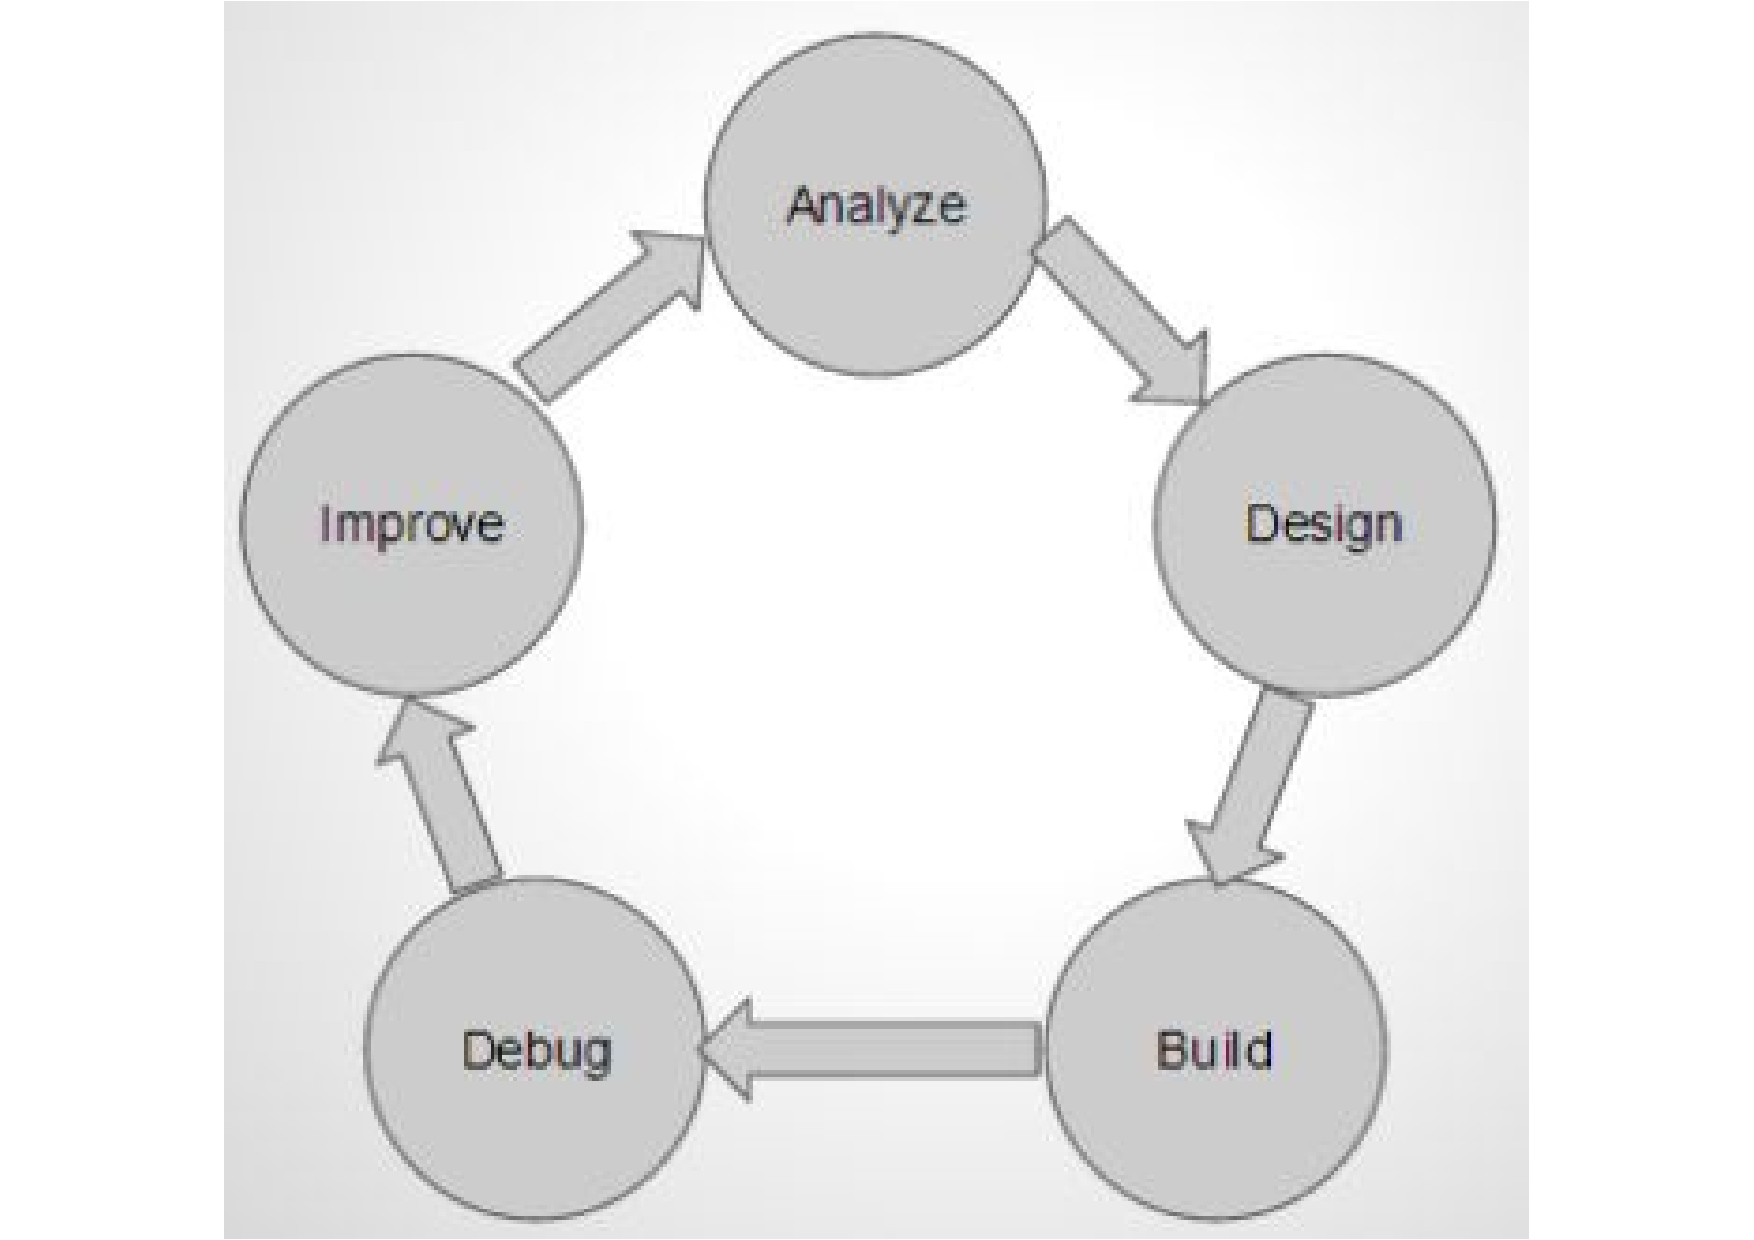
\includegraphics[scale=.3]{figures/approach.pdf}
		\caption{Approach Diagram} 
	\end{figure}	
\end{frame}
%--
\begin{frame}
	\frametitle{Design}
	\begin{columns}[T]
		\begin{column}{0.5\textwidth}
			\begin{block}{2D Drawing}
				\begin{figure}
				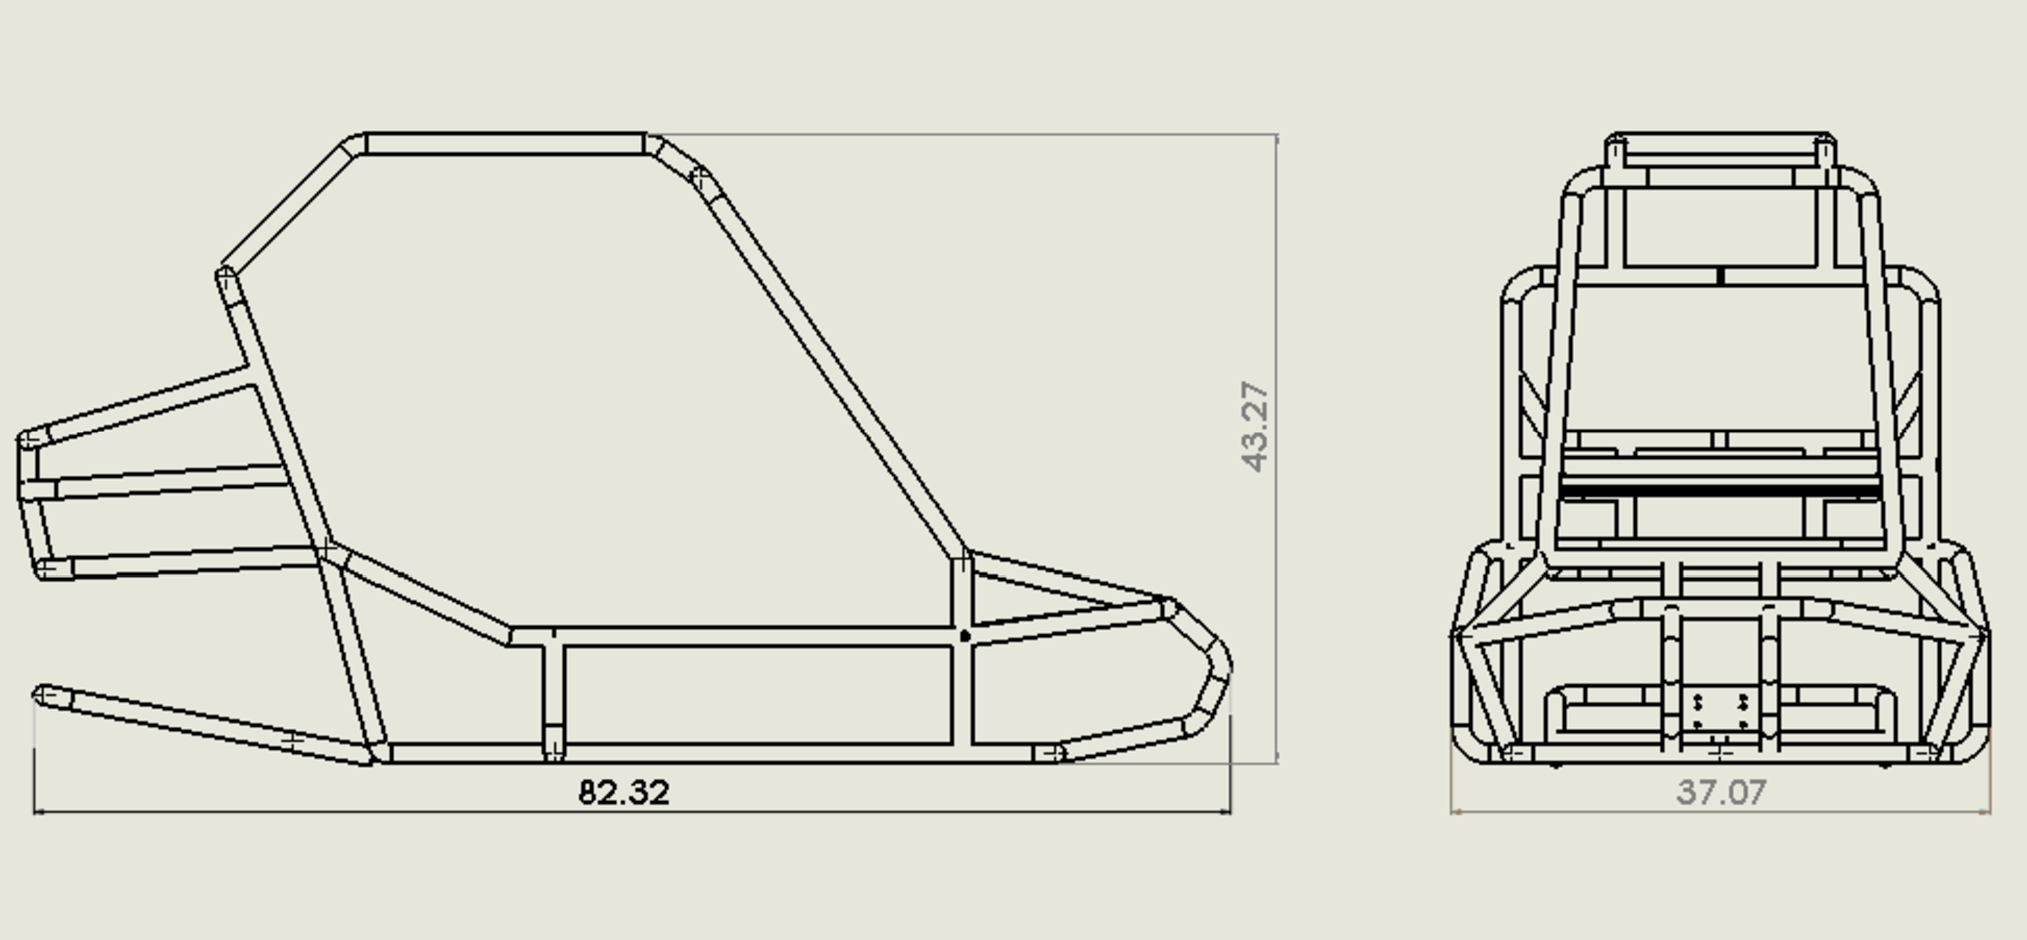
\includegraphics[scale=.16]{figures/chassis_model.pdf}
				\caption {Initial 2D Chassis Drawing}
				\end{figure}
			\end{block}
		\end{column}
		\begin{column}{0.5\textwidth}
			\begin{block}{3D Model}
				\begin{figure}
				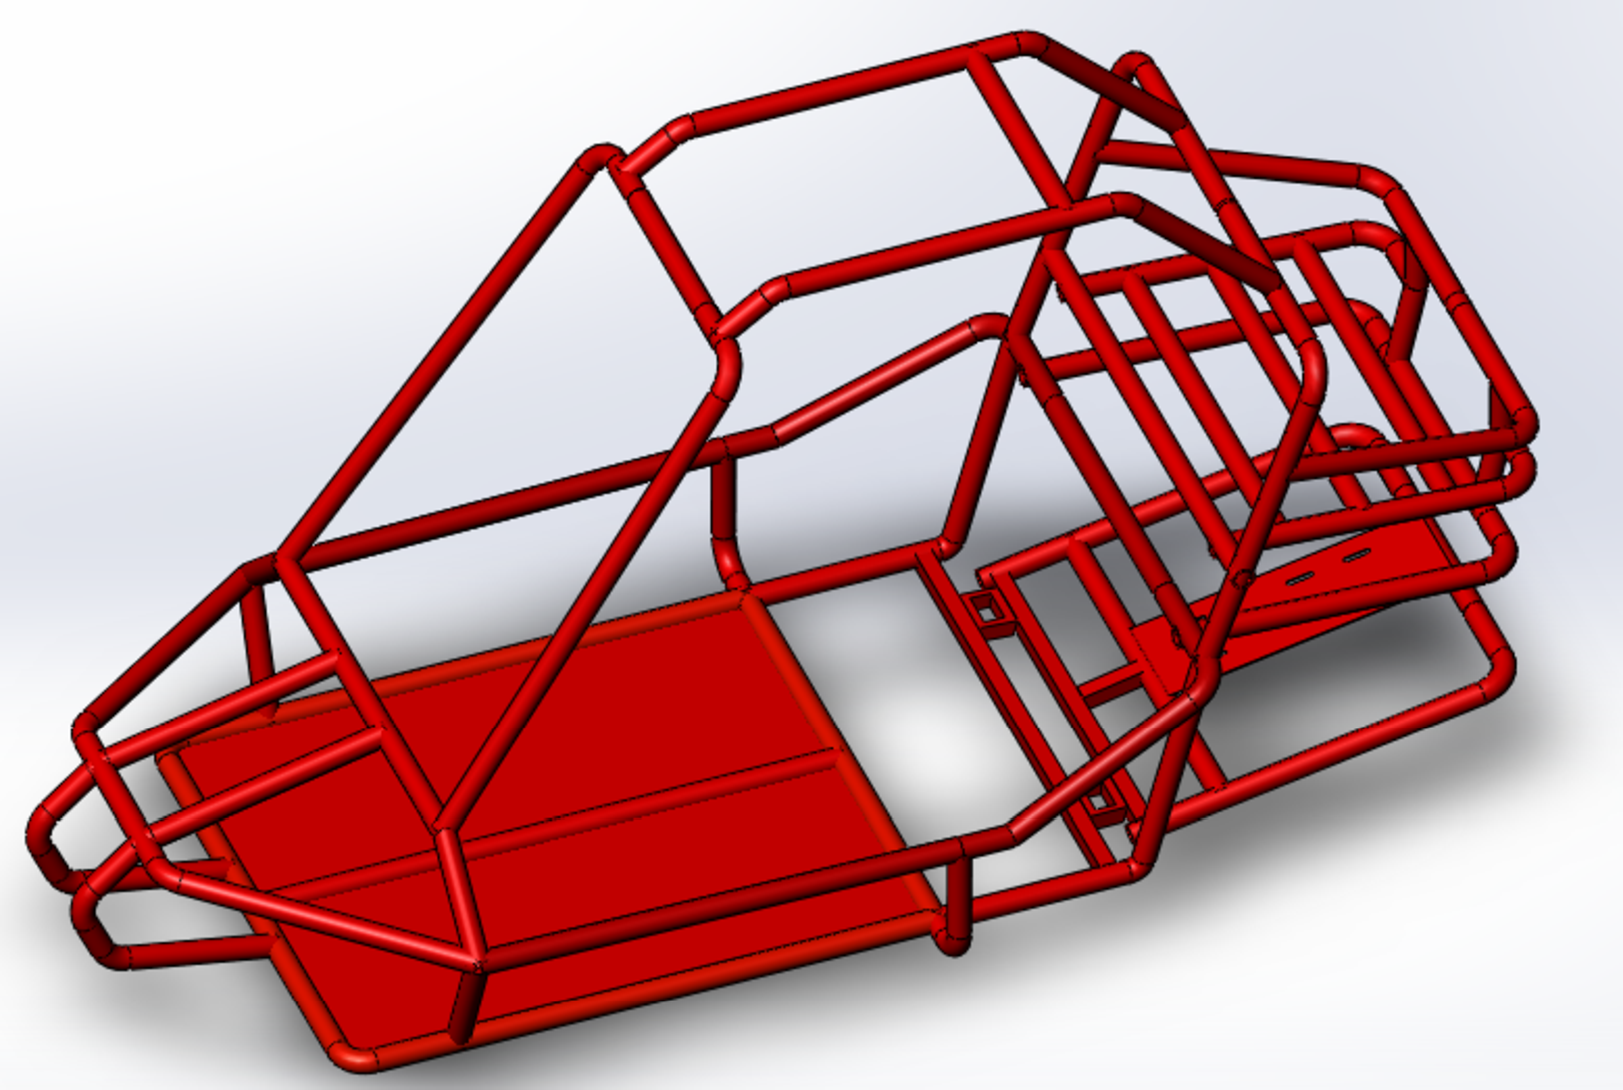
\includegraphics[scale=.14]{figures/solidwork_model.pdf}
				\caption {Initial 3D Chassis Design}
				\end{figure}
			\end{block}
		\end{column}
	\end{columns}	
\end{frame}			
%--
\begin{frame}
	\frametitle{Build}
		\begin{itemize}
			\item Acquire parts within budget
			\item Construct a drivetrain
			\item Implement a control system
			\item Retain a sufficient level of safety for the driver
		\end{itemize}
\end{frame}
%--
\begin{frame}
	\frametitle{Team Management}
		\begin{block}{Fabrication \& Mechanical}
			\begin{itemize}
				\item Responsible for carrying out all mechanical operations necessary to create a working vehicle
				\item Chassis modification to satisfy the requirements
			\end{itemize}
		\end{block}
		\begin{block}{Electrical}
			\begin{itemize}
				\item Responsible for research, procurement, and implementation of sensors, a microcontroller, motors, and programmable motor controllers
			\end{itemize}
		\end{block}
		\begin{block}{Programming \& Controls}
			\begin{itemize}
			\item Responsible for implementing the algorithms necessary to achieve 		differential control
			\item Programming code to take sensor input and produce a controlled output
			\end{itemize}
		\end{block}
\end{frame}
%==================================================================================
\section{Mechanical}
%--
\begin{frame}
	\frametitle{Mechanical}
		\begin{block}{Chassis}
			\begin{itemize}
				\item Repair
				\item Retrofitting
				\item Brakes
			\end{itemize}
		\end{block}
		\begin{block}{Battery Box}
			\begin{itemize}
				\item Seat
				\item Safety
				\item Control Panel
			\end{itemize}
		\end{block}
		\begin{block}{Motors}
			\begin{itemize}
				\item Motor Mounts
				\item Chain Drive
			\end{itemize}
		\end{block}		
\end{frame}	
%--
\begin{frame}
	\frametitle{Chassis Repair and Fabrication}
	\begin{figure}
		\centering 
		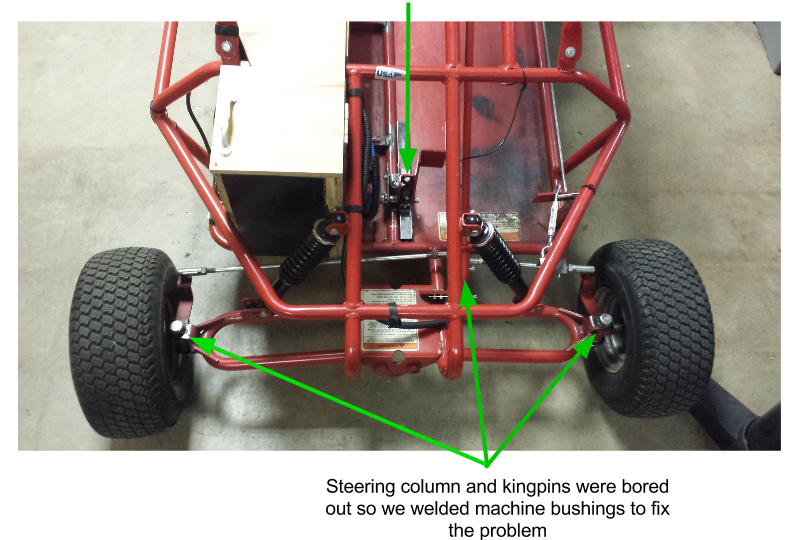
\includegraphics[scale=.3]{figures/png/SeniorDesignPresentation-1.png}
		\caption{Front End Repairs} 
	\end{figure}	
\end{frame}
%--
\begin{frame}
	\frametitle{Chassis Repair and Fabrication}
	\begin{figure}
		\centering 
		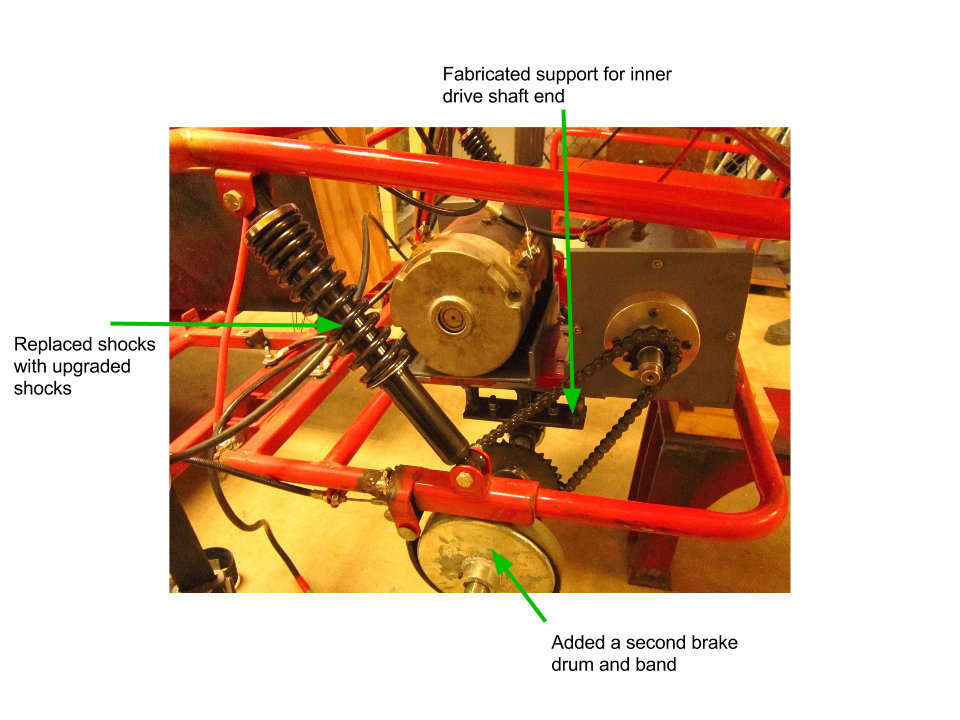
\includegraphics[scale=.3]{figures/png/SeniorDesignPresentation-3.png}
		\caption{Rear End Repairs} 
	\end{figure}	
\end{frame}
%--
\begin{frame}
	\frametitle{Chassis Repair and Fabrication}
	\begin{figure}
		\centering 
		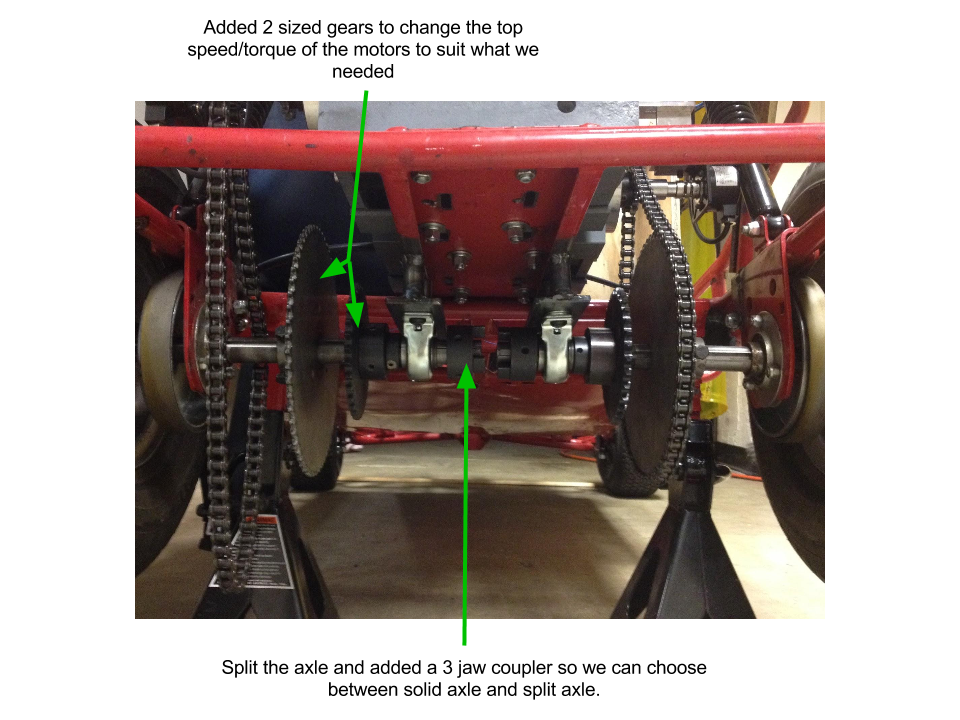
\includegraphics[scale=.27]{figures/png/SeniorDesignPresentation-4.png}
		\caption{Rear End Repairs 2} 
	\end{figure}	
\end{frame}
%--
\begin{frame}
	\frametitle{Motors}
	\begin{columns}[T]
		\begin{column}{0.5\textwidth}
			\begin{block}{Motor}
				\begin{figure}
					\centering 
					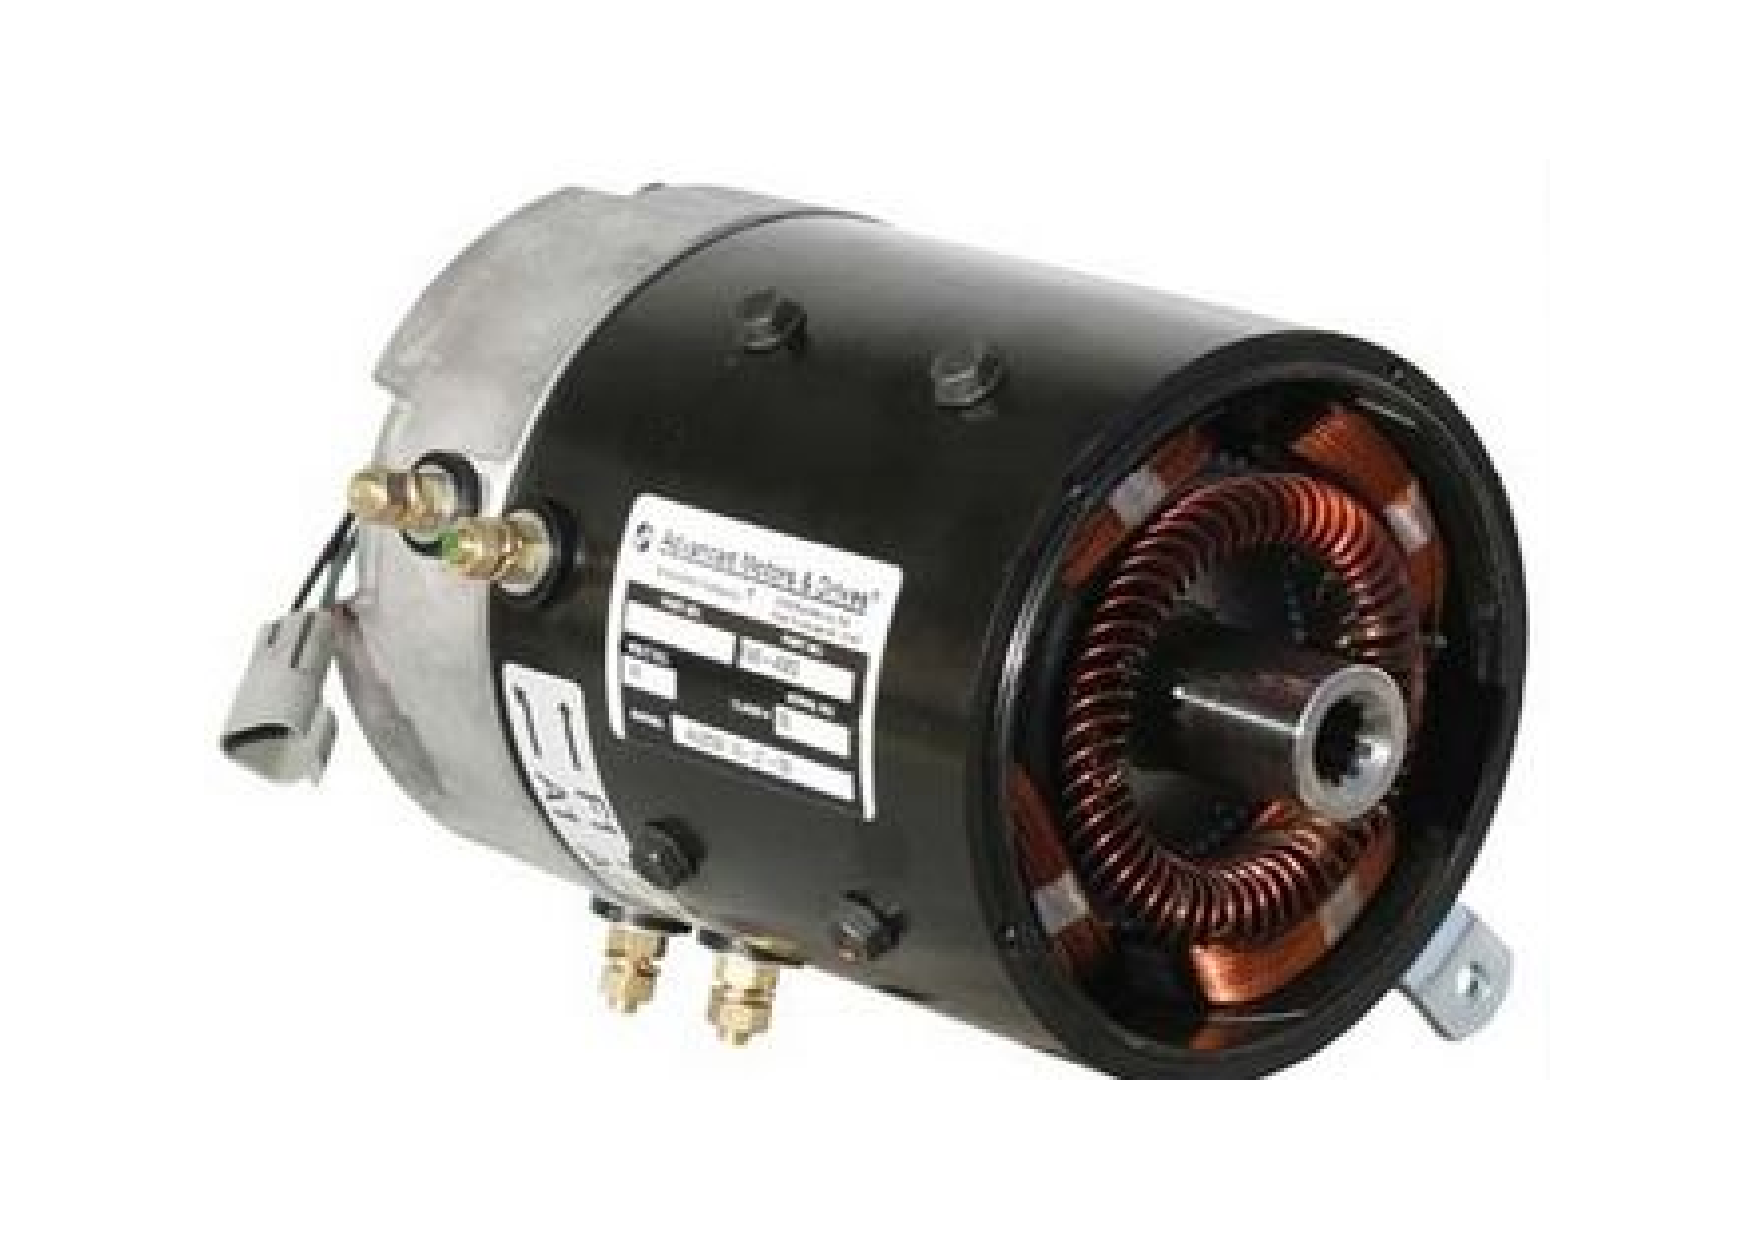
\includegraphics[scale=.2]{figures/motorpic.pdf}
					\caption{Advanced D.C. Motors} 
				\end{figure}
			\end{block}
		\end{column}		
		\begin{column}{0.5\textwidth}
			\begin{block}{Motor Information}
				\begin{itemize}
					\item Motor manufactured by Advanced D.C. Motors
					\item Sepex (shunt wound) motor design
					\item 36 volt maximum input
				\end{itemize}
			\end{block}	
		\end{column}
	\end{columns}							
\end{frame}
%--
\begin{frame}
	\frametitle{Motors}
	\begin{figure}
		\centering 
		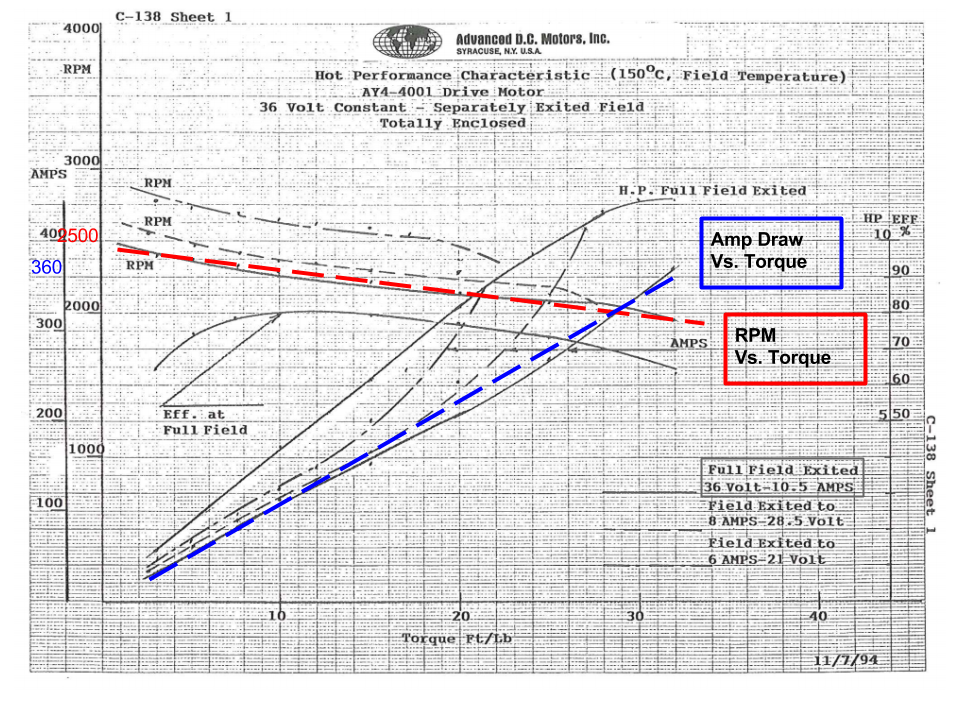
\includegraphics[scale=.30]{figures/png/SeniorDesignPresentation-5.png} 
	\end{figure}	
\end{frame}
%--
\begin{frame}
	\frametitle{Battery Box}
	\begin{figure}
		\centering 
		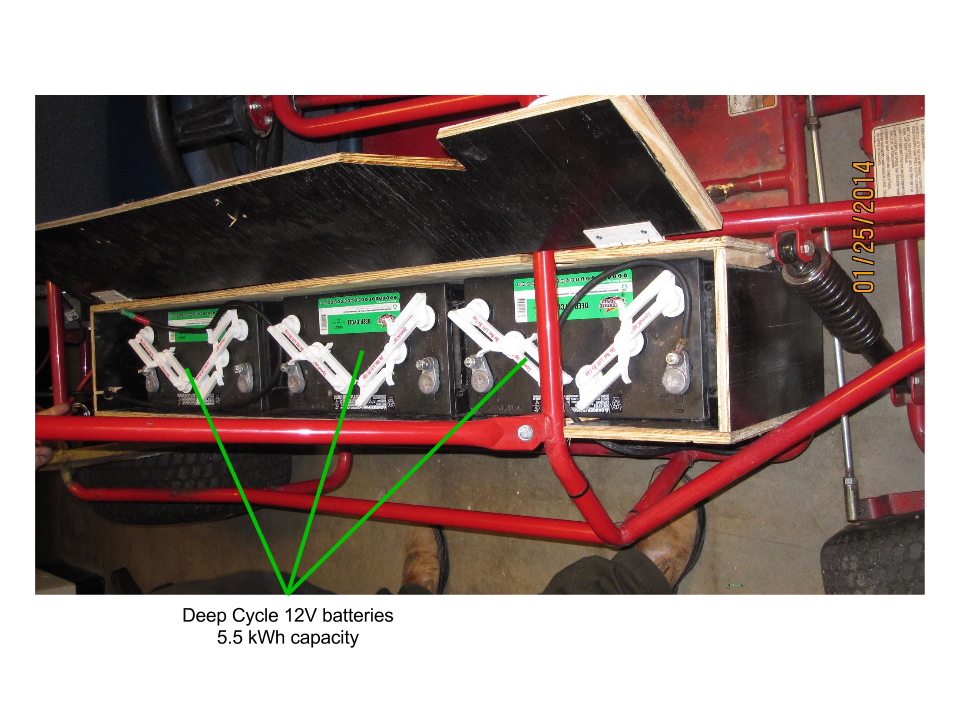
\includegraphics[scale=.3]{figures/png/SeniorDesignPresentation-6.png}
		\caption{Battery Box} 
	\end{figure}	
\end{frame}
%--
\begin{frame}
	\frametitle{Cockpit}
	\begin{figure}
		\centering 
		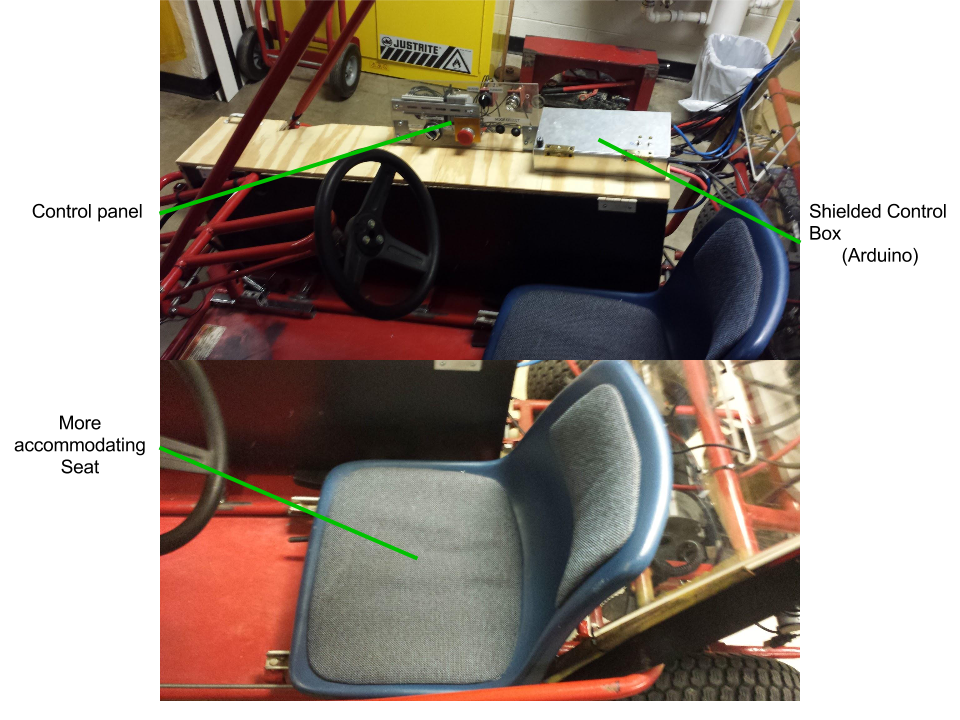
\includegraphics[scale=.27]{figures/png/SeniorDesignPresentation-7.png} 
	\end{figure}	
\end{frame}
%==================================================================================
\section{Electrical}
%--
\begin{frame}
	\frametitle{Electrical}
		\begin{block}{Arduino Due}
			\begin{itemize}
				\item Advantages
				\item Implementation
			\end{itemize}
		\end{block}
		\begin{block}{Op-Amp Circuitry}
			\begin{itemize}
				\item Reasons needed and design
				\item Resistance calculations
			\end{itemize}
		\end{block}
		\begin{block}{Control Panel}
			\begin{itemize}
				\item Solenoids
			\end{itemize}
		\end{block}		
\end{frame}	
%--
\begin{frame}
	\frametitle{Control Panel}
	\begin{columns}[T]
		\begin{column}{0.5\textwidth}
			\begin{block}{Panel Drawing}
				\begin{figure}
					\centering 
					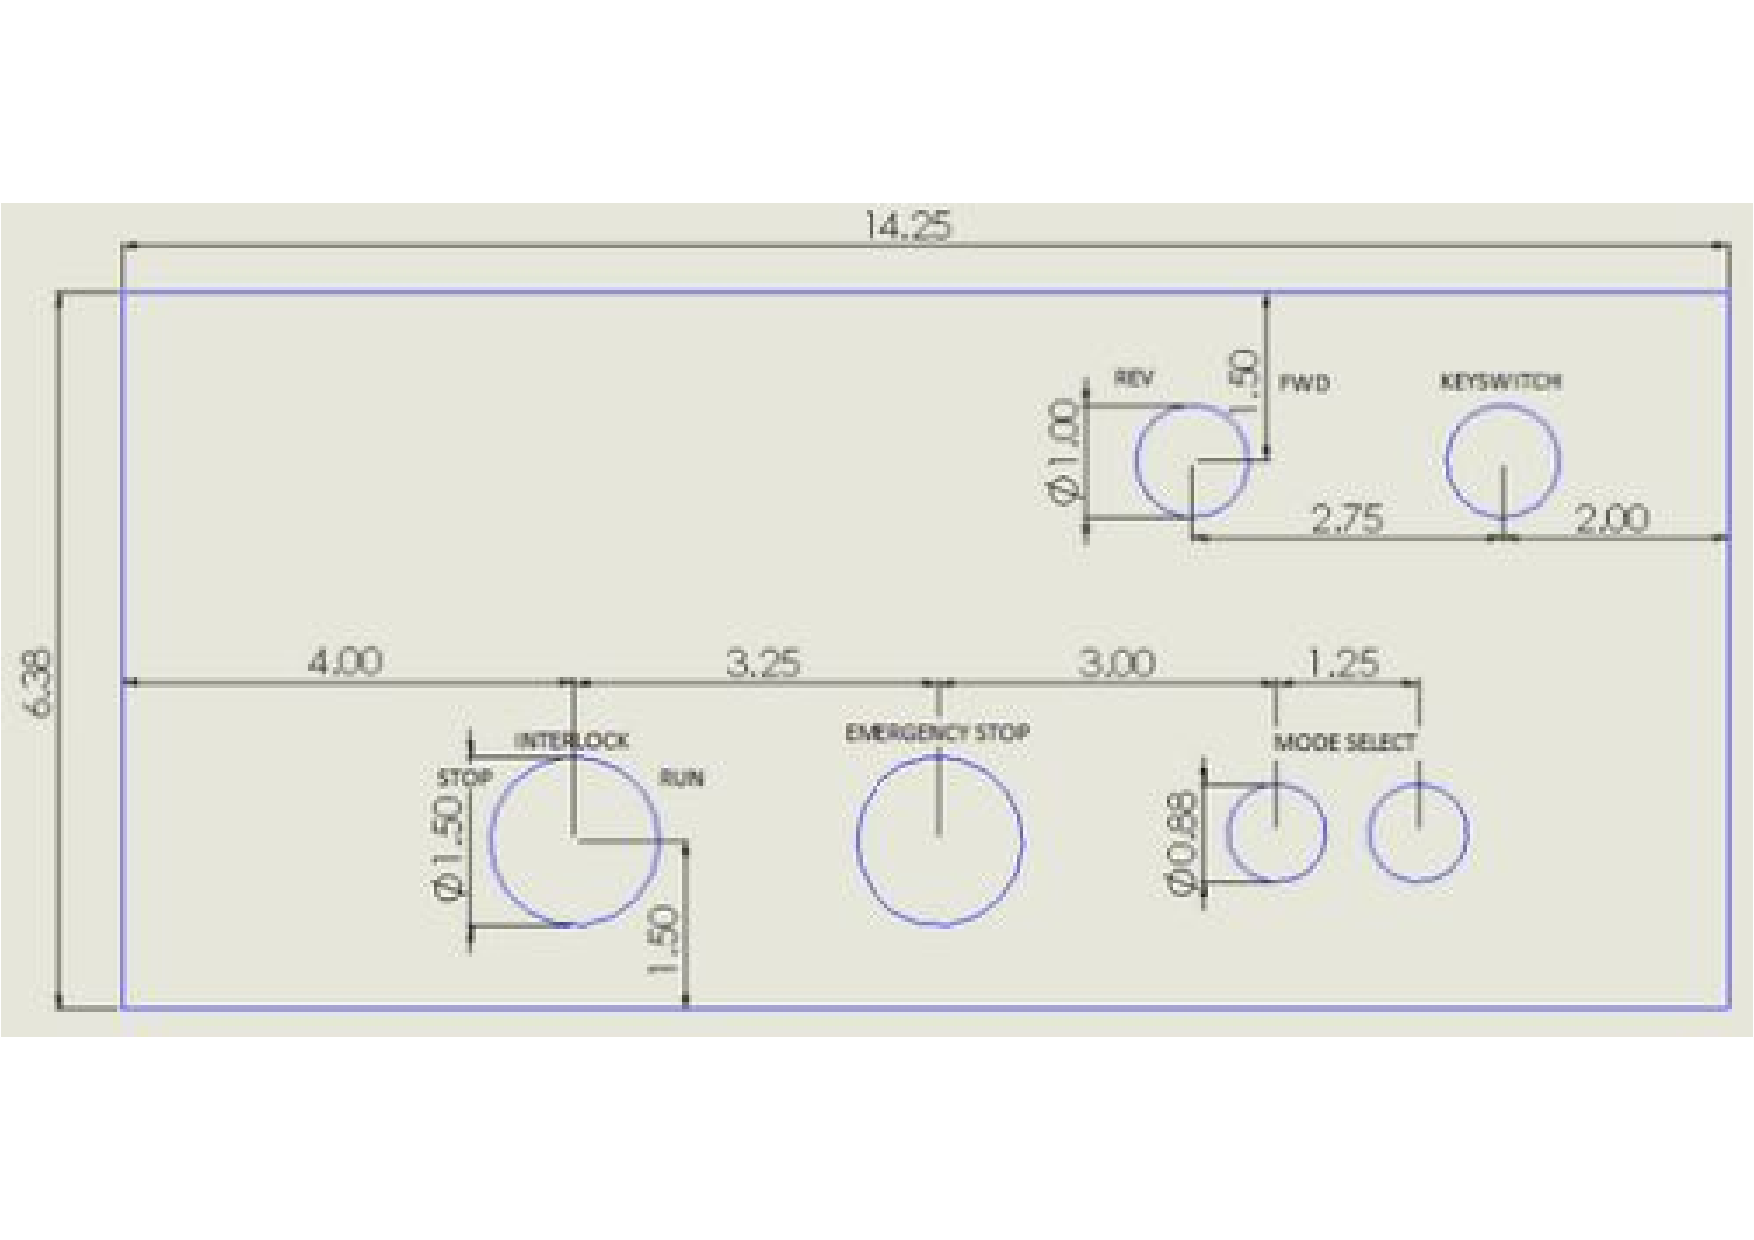
\includegraphics[scale=.18]{figures/panel2.pdf} 
				\end{figure}
			\end{block}
		\end{column}		
		\begin{column}{0.5\textwidth}
			\begin{block}{Panel Rendering}
				\begin{figure}
					\centering
					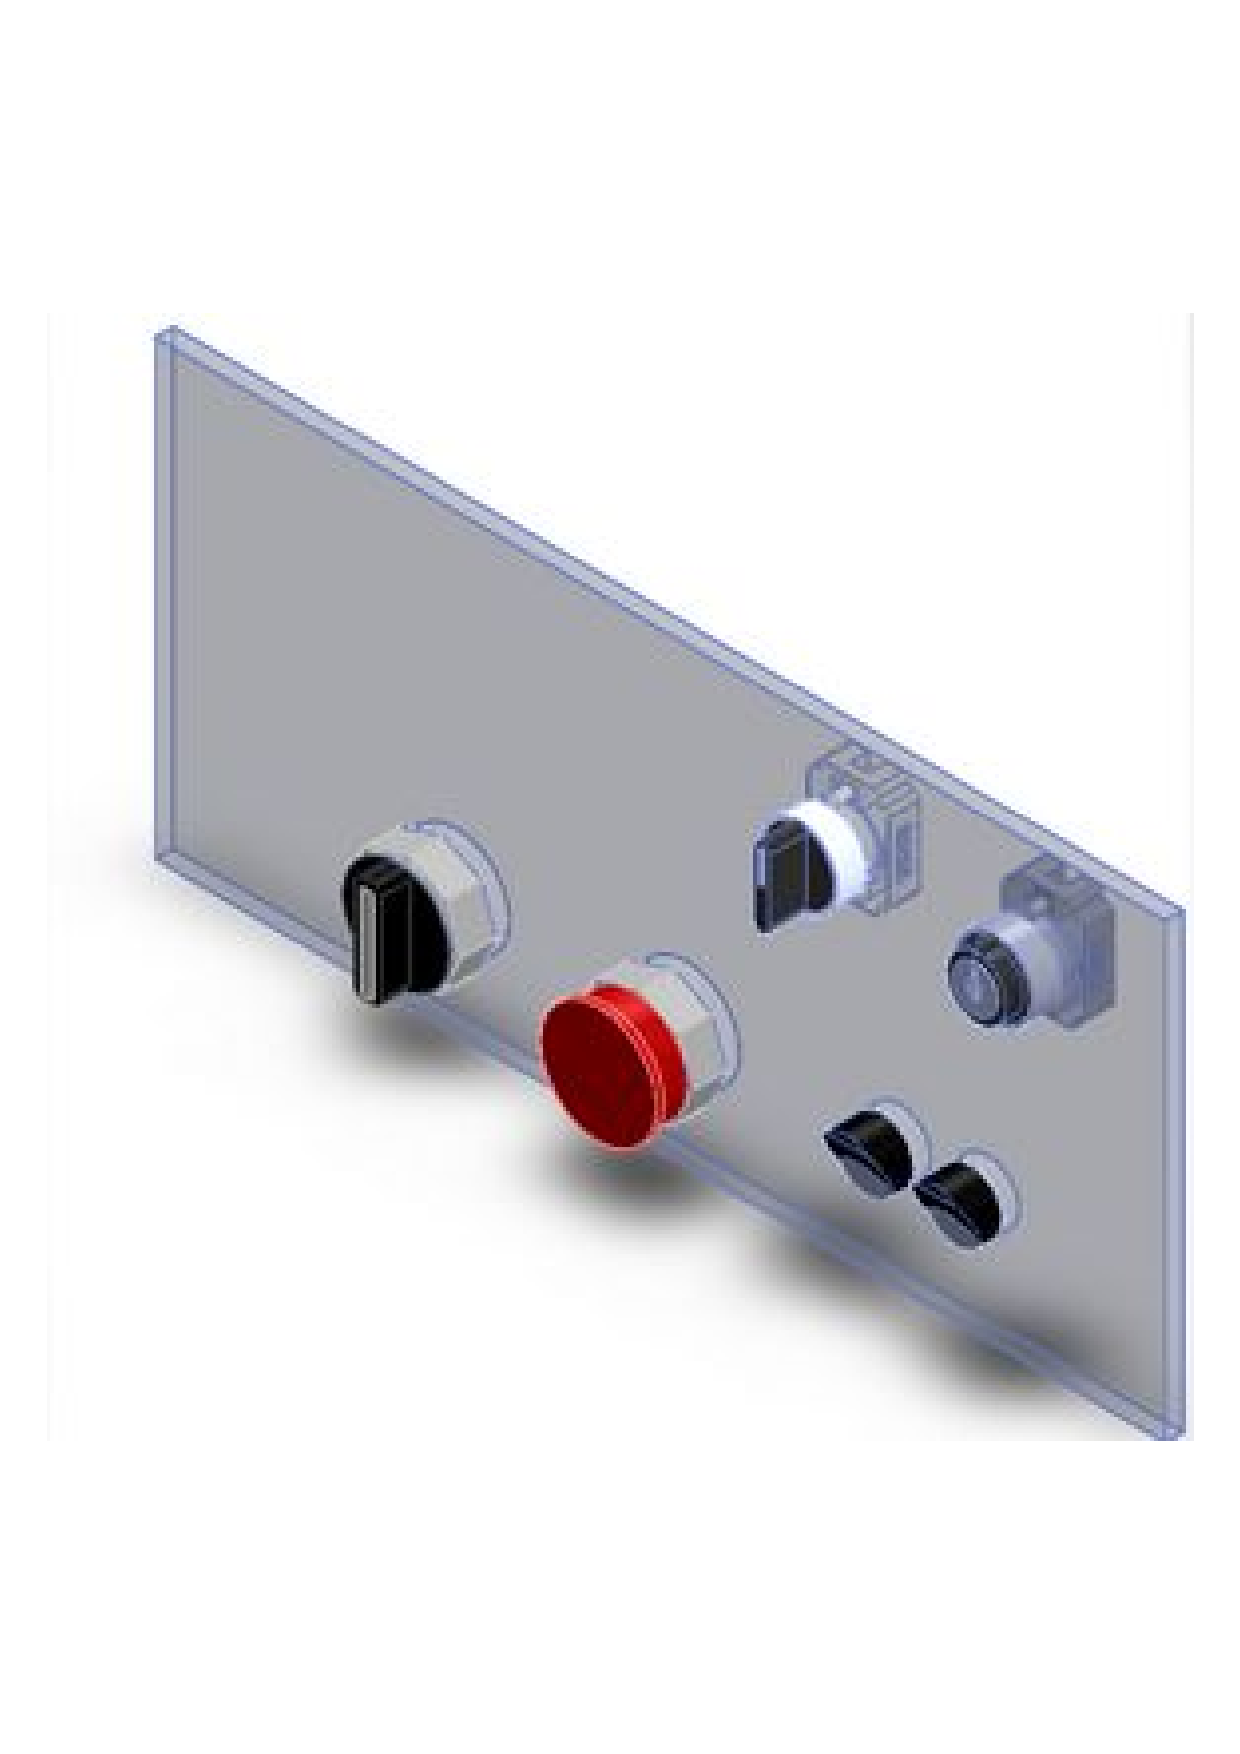
\includegraphics[scale=.2]{figures/panel1.pdf}
				\end{figure}
			\end{block}	
		\end{column}
	\end{columns}							
\end{frame}
%--
\begin{frame}
	\frametitle{Control Panel}
	\begin{figure}
		\centering 
		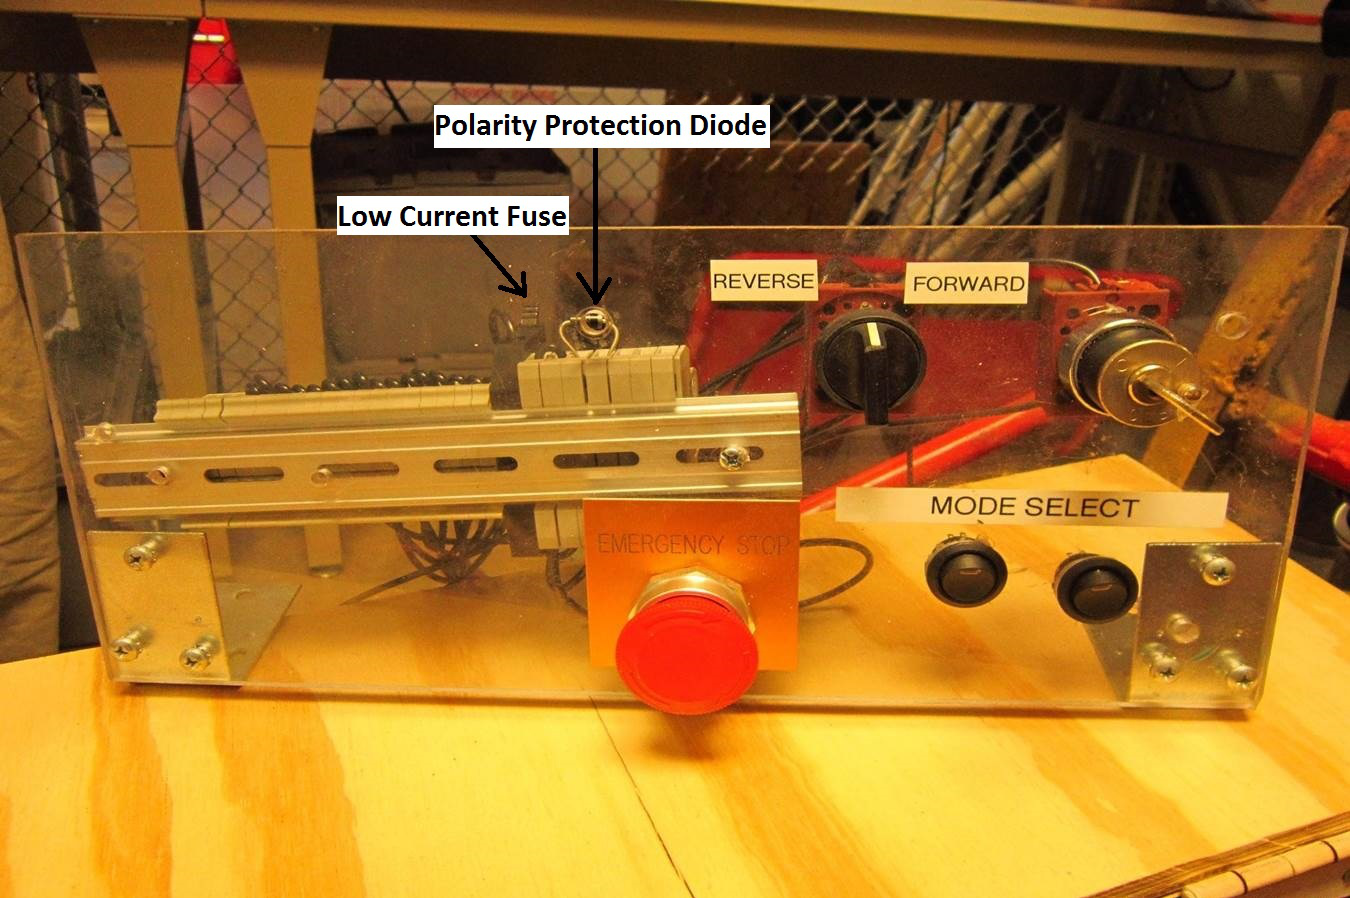
\includegraphics[scale=.32]{figures/panel-update.pdf}
		\caption{Finished Control Panel}
	\end{figure}	
\end{frame}
%--
\begin{frame}
	\frametitle{Main Contactors \& Solenoids}
	\begin{figure}
		\centering 
		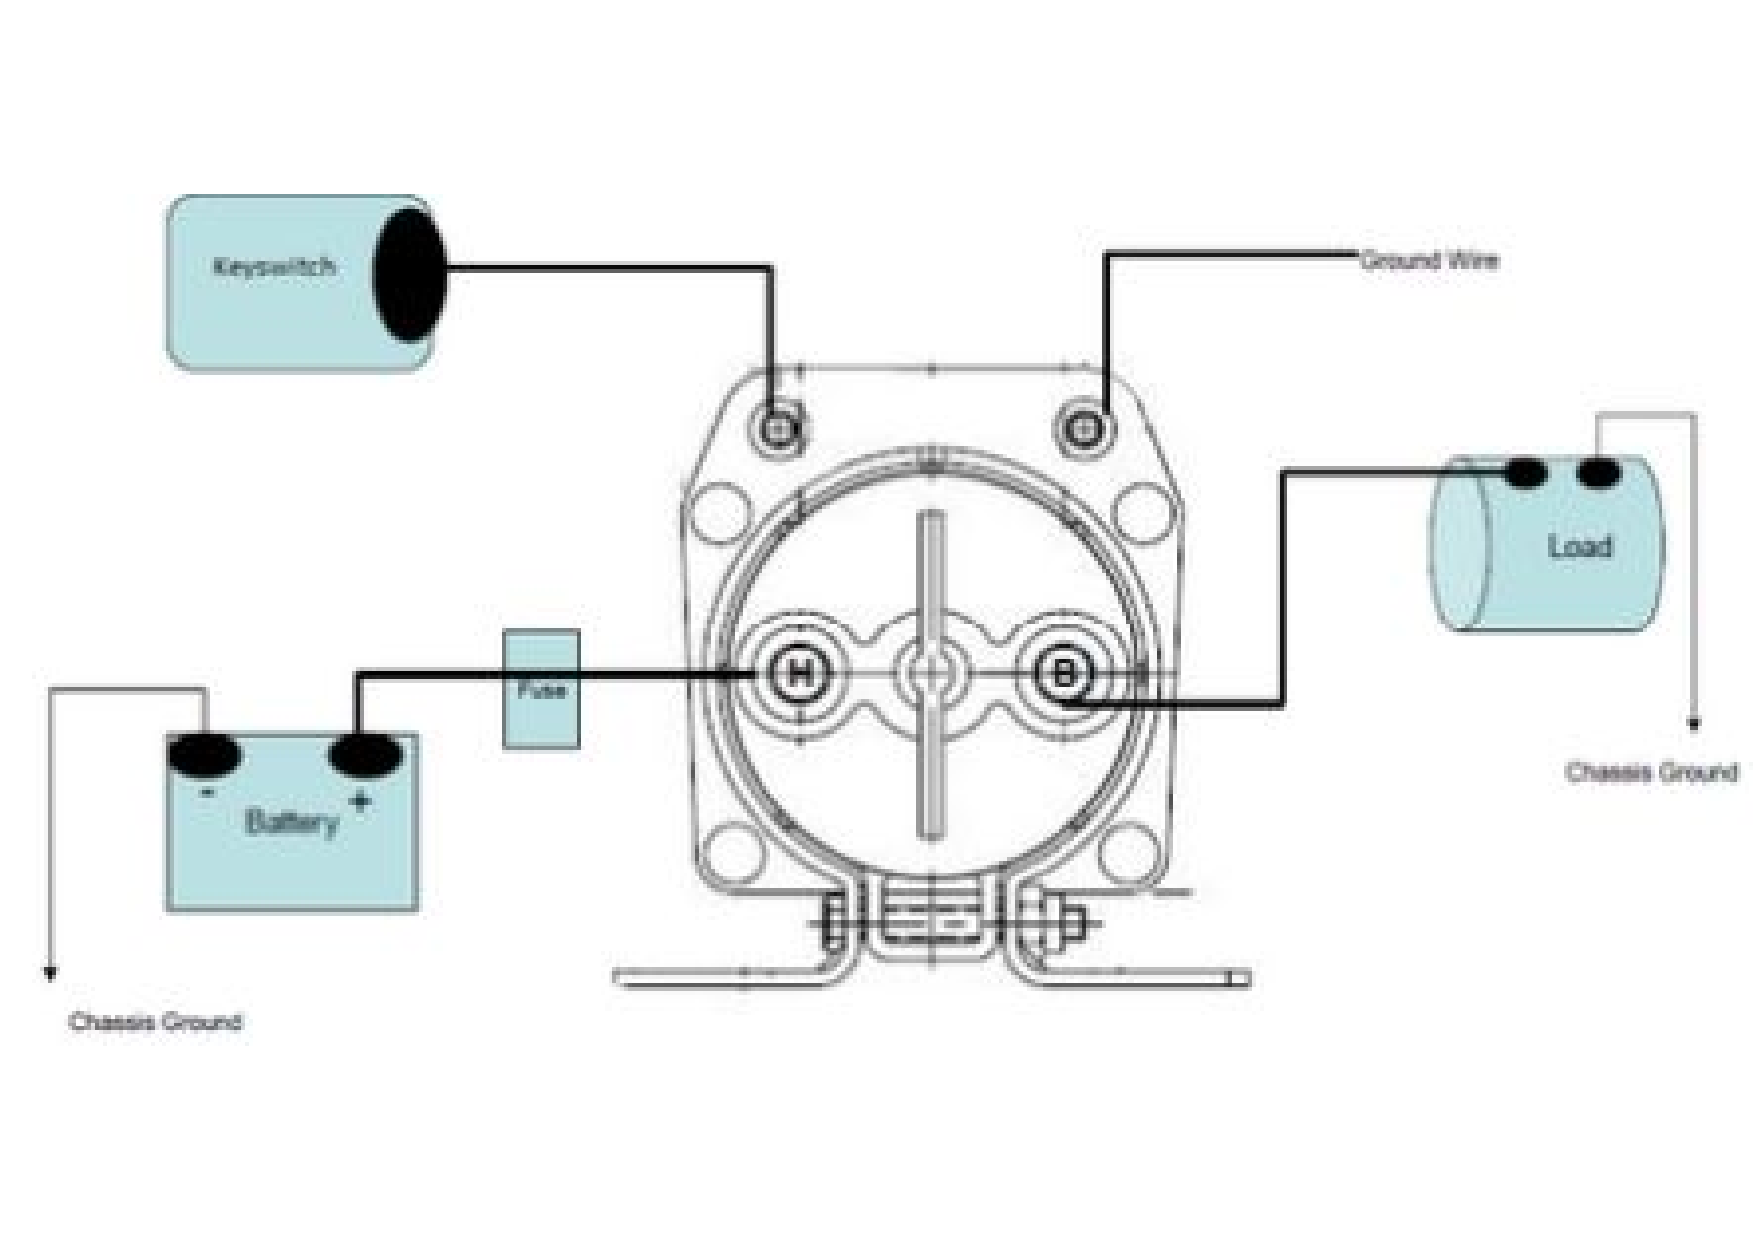
\includegraphics[scale=.30]{figures/panel4.pdf}
		\caption{Solenoid Schematic}
	\end{figure}	
\end{frame}
%--
\begin{frame}
	\frametitle{Curtis Motor Controllers}
	\begin{figure}
		\centering 
		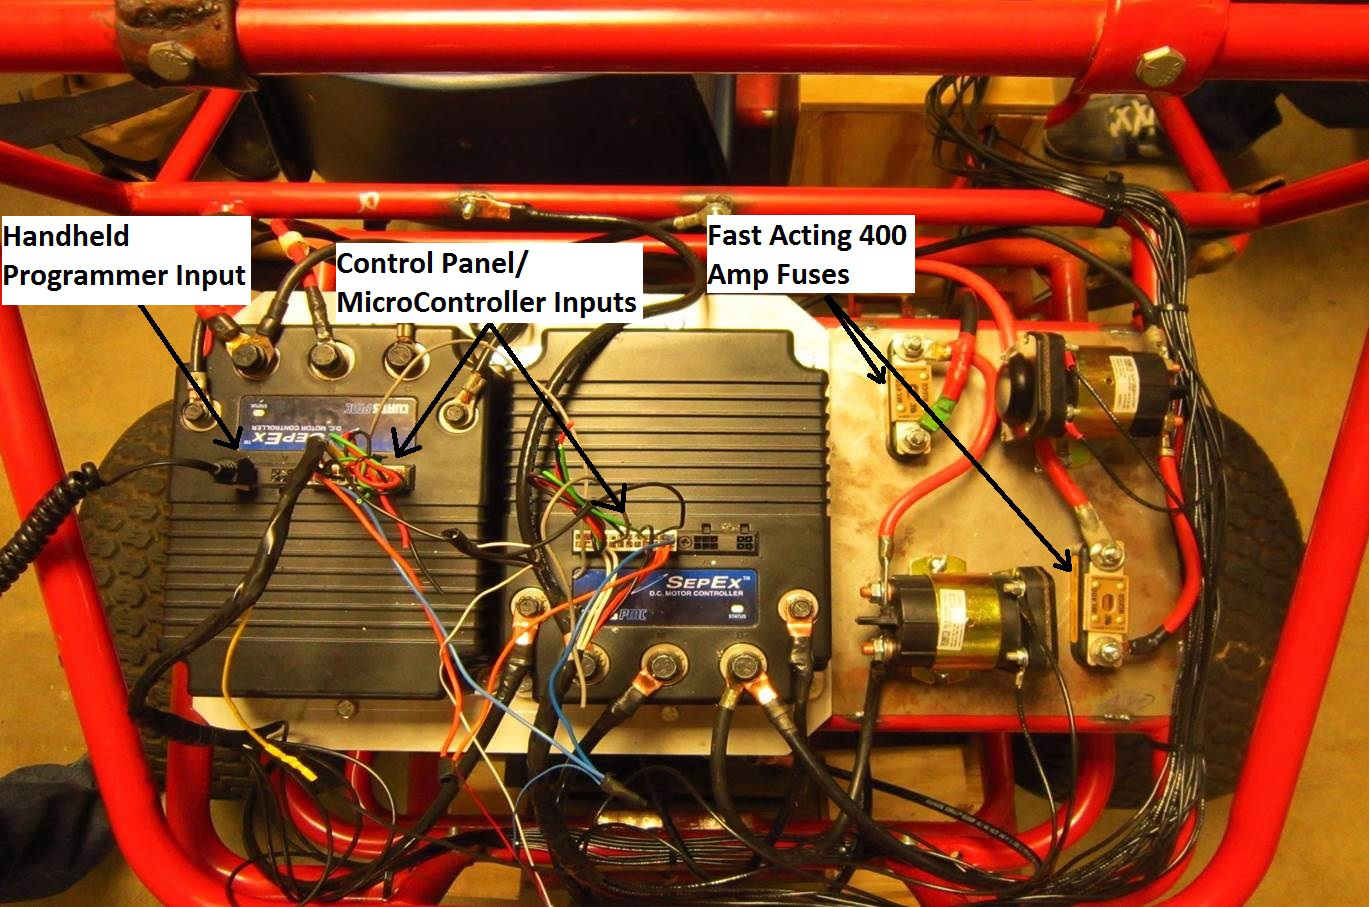
\includegraphics[scale=.35]{figures/curtis1.pdf}
		\caption{Curtis Controllers}
	\end{figure}	
\end{frame}
%--
\begin{frame}
	\frametitle{Arduino Due}
	\begin{figure}
		\centering 
		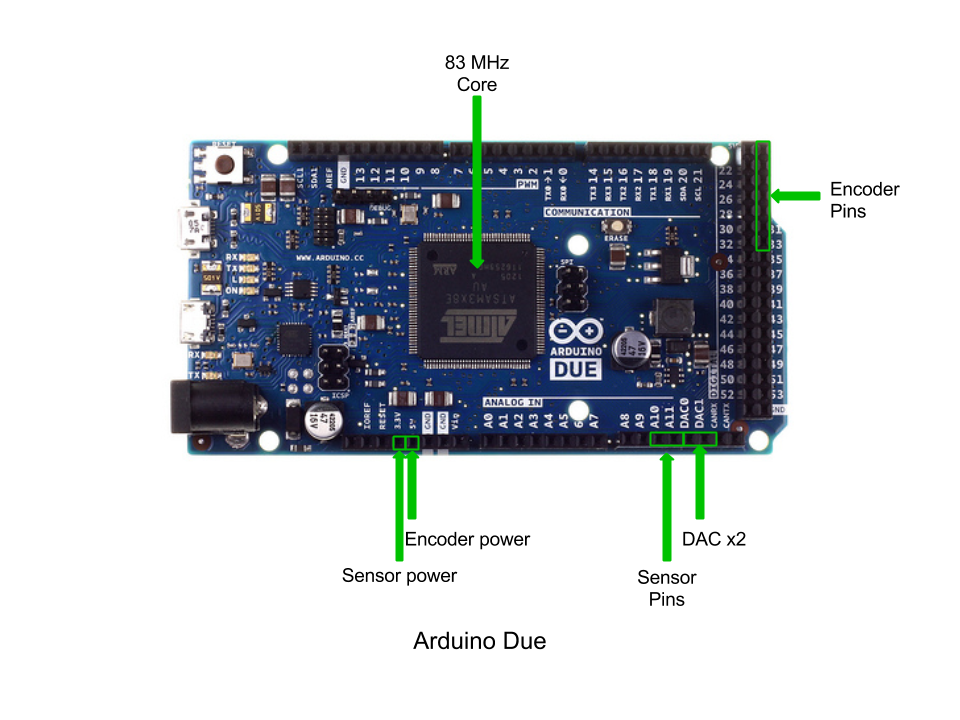
\includegraphics[scale=.27]{figures/png/SeniorDesignPresentation-9.png}
		\caption{Arduino Due}
	\end{figure}	
\end{frame}
%--
\begin{frame}
	\frametitle{Arduino Due}
	\begin{figure}
		\centering 
		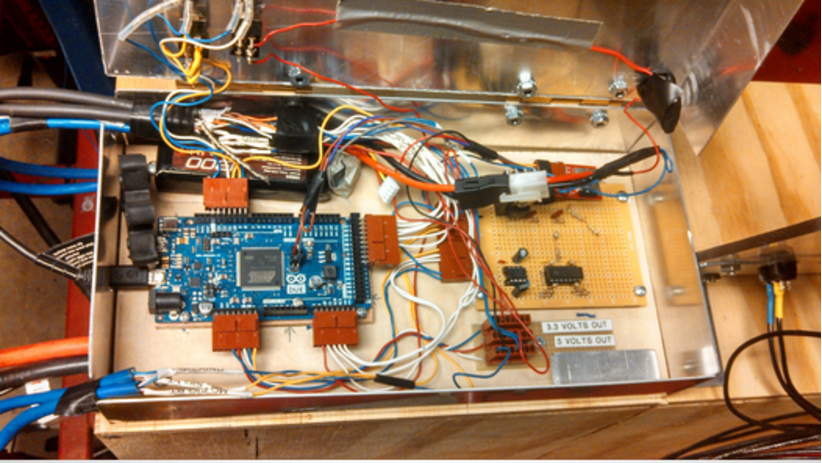
\includegraphics[scale=.7]{figures/arduino2.pdf}
		\caption{Arduino Due}
	\end{figure}	
\end{frame}
%--
\begin{frame}
	\frametitle{Op Amp Circuit}
		\begin{block}{Intended Purpose}
			\begin{itemize}
				\item Fix voltage range problem
			\end{itemize}
		\end{block}
		\begin{block}{Design Implementation}
			\begin{itemize}
				\item Inverting amplifier
				\item Summing amplifier
			\end{itemize}
		\end{block}
		\begin{block}{Problems Encountered}
			\begin{itemize}
				\item Arduino pin needed converting to negative voltage
				\item Back current
			\end{itemize}
		\end{block}		
\end{frame}
%--
\begin{frame}
	\frametitle{Op Amp Circuit}
	\begin{columns}[T]
		\begin{column}{0.5\textwidth}
			\begin{block}{Inverting Amplifier}
				\begin{figure}
					\centering 
					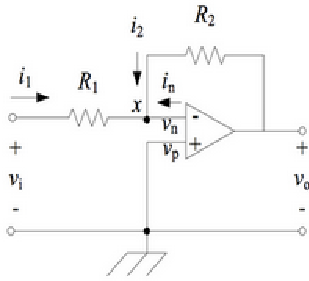
\includegraphics[scale=.7]{figures/opamp1-1.pdf} 
				\end{figure}
			\end{block}
		\end{column}		
		\begin{column}{0.5\textwidth}
			\begin{block}{Summing Amplifier}
				\begin{figure}
					\centering
					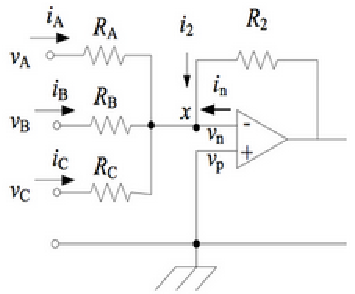
\includegraphics[scale=.7]{figures/opamp2-2.pdf}
				\end{figure}
			\end{block}	
		\end{column}
	\end{columns}
	\begin{block}{Related Equations}
		\begin{figure}
			\centering
			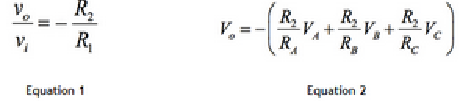
\includegraphics[scale=.6]{figures/opamp3-3.pdf}
		\end{figure}
	\end{block}								
\end{frame}
%--
\begin{frame}
	\frametitle{Op Amp Circuit}
	\begin{figure}
		\centering 
		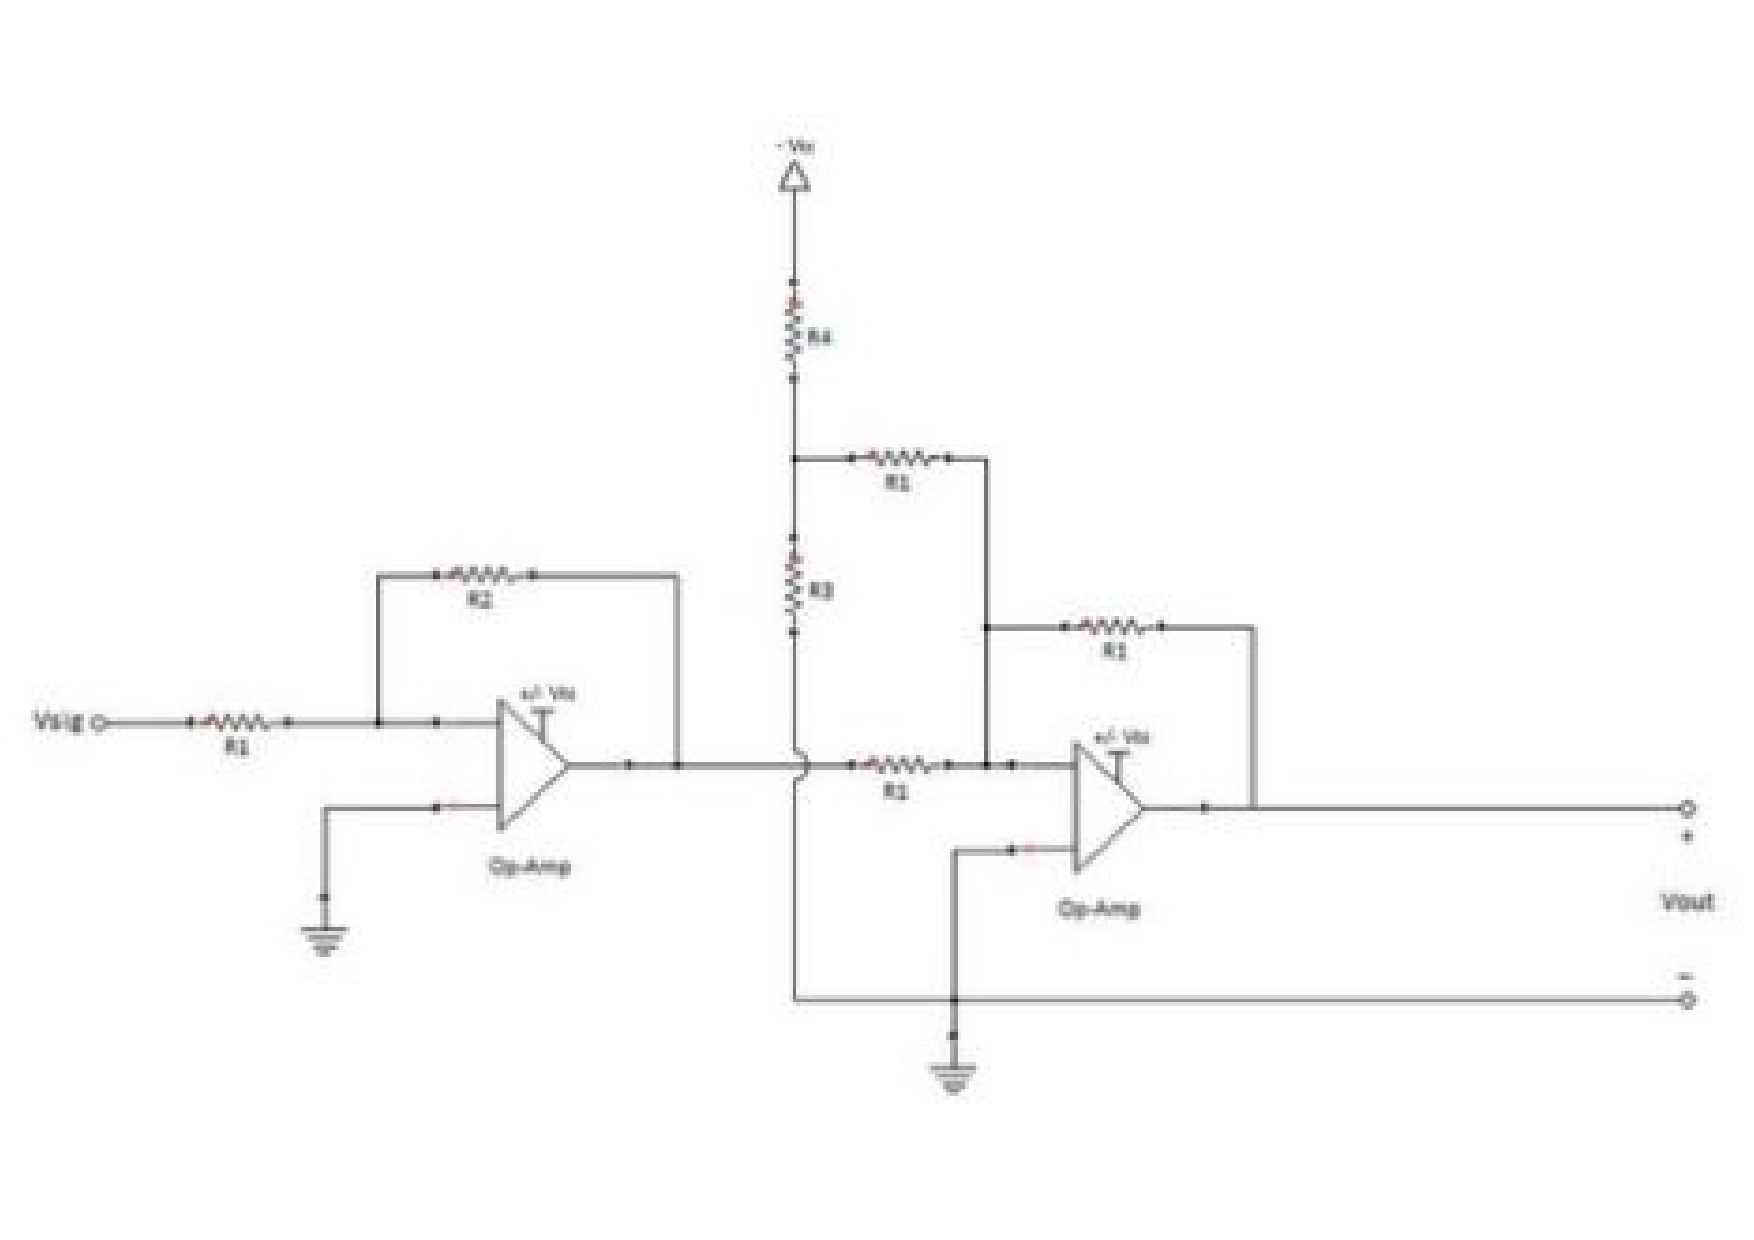
\includegraphics[scale=.3]{figures/opampfinal.pdf}
		\caption{Final Op Amp Design}
	\end{figure}	
\end{frame}
%--
\begin{frame}
	\frametitle{Op Amp Circuit}
	\begin{columns}[T]
		\begin{column}{0.5\textwidth}
			\begin{block}{Negative Voltage Implementation}
				\begin{figure}
					\centering 
					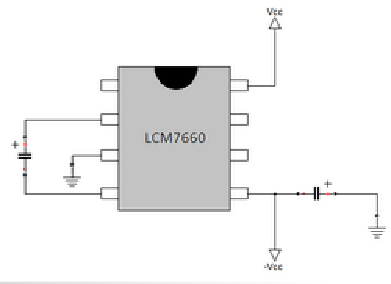
\includegraphics[scale=.7]{figures/ckt1.pdf} 
				\end{figure}
			\end{block}
		\end{column}		
		\begin{column}{0.5\textwidth}
			\begin{block}{Op-Amp Circuit Implementation}
				\begin{figure}
					\centering
					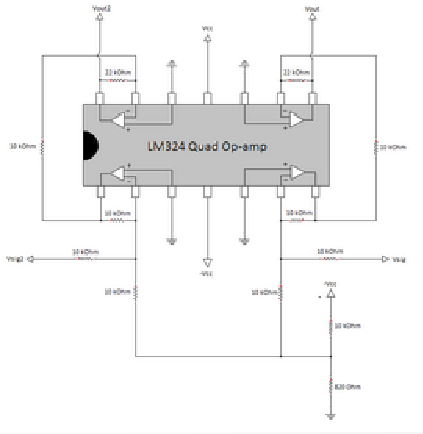
\includegraphics[scale=.7]{figures/ckt2.pdf}
				\end{figure}
			\end{block}	
		\end{column}
	\end{columns}						
\end{frame}
%--
\begin{frame}
	\frametitle{Op Amp Circuit}
	\begin{figure}
		\centering 
		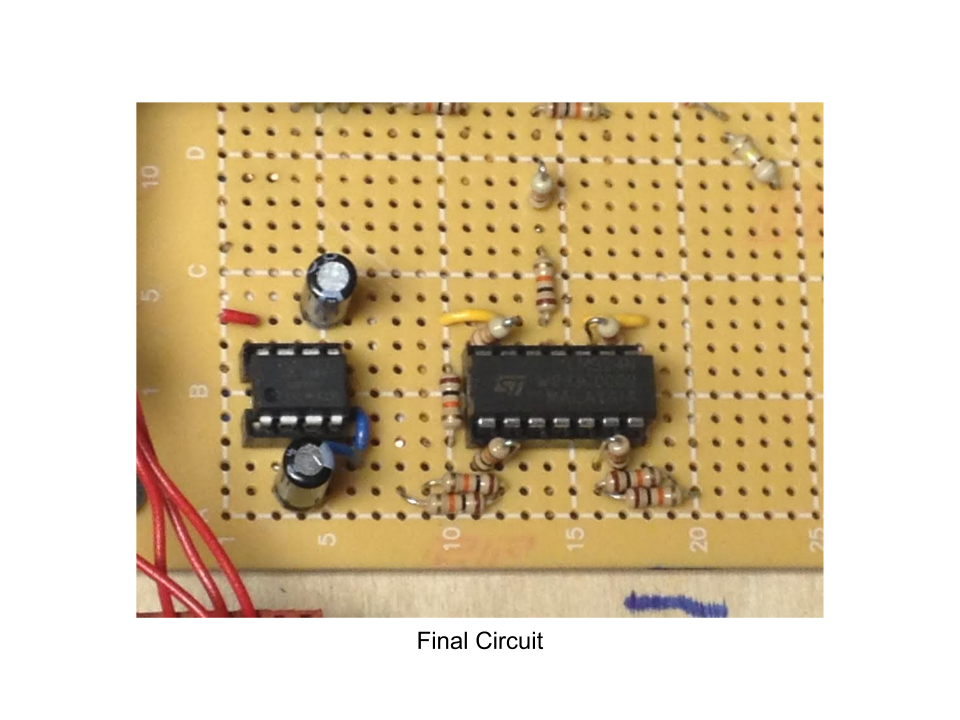
\includegraphics[scale=.3]{figures/png/SeniorDesignPresentation-2.png}
		\caption{Op-Amp Breadboard Design}
	\end{figure}	
\end{frame}
%================================================================================
\section{Controls}
%--
\begin{frame}
	\frametitle{Control}
		\begin{block}{Equations of Motion}
			\begin{itemize}
				\item Ackermann steering
				\item Hierarchy of control
			\end{itemize}
		\end{block}
		\begin{block}{Sensors}
			\begin{itemize}
				\item Throttle
				\item Steering angle
				\item Wheel speed
			\end{itemize}
		\end{block}
		\begin{block}{Programming \& Data Collection}
			\begin{itemize}
				\item Throttle
				\item Steering
				\item Encoders
				\item Differential
			\end{itemize}
		\end{block}		
\end{frame}
%--
\begin{frame}
	\frametitle{Equations of Motion}
	\begin{columns}[T]
		\begin{column}{0.5\textwidth}
			\begin{block}{Ackermann Steering}
				\begin{figure}
					\centering 
					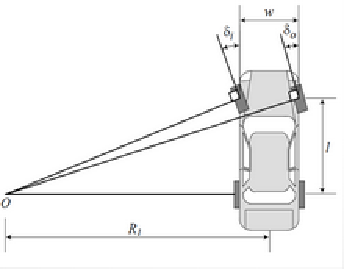
\includegraphics[scale=.7]{figures/ackermann2.pdf} 
				\end{figure}
			\end{block}
		\end{column}		
		\begin{column}{0.5\textwidth}
			\begin{block}{Ackermann Geometry}
				\begin{figure}
					\centering
					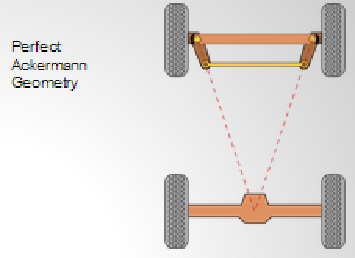
\includegraphics[scale=.7]{figures/ackermann3.pdf}
				\end{figure}
			\end{block}	
		\end{column}
	\end{columns}
	\begin{block}{Related Equations}
		\begin{figure}
			\centering
			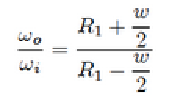
\includegraphics[scale=.6]{figures/ackermann4.pdf}
			\\
			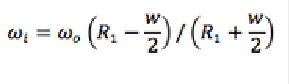
\includegraphics[scale=.6]{figures/ackermann5.pdf}
		\end{figure}
	\end{block}								
\end{frame}
%--
\begin{frame}
	\frametitle{Control System Description}
		\begin{block}{Control Block Diagram}
			\begin{figure}
				\centering
				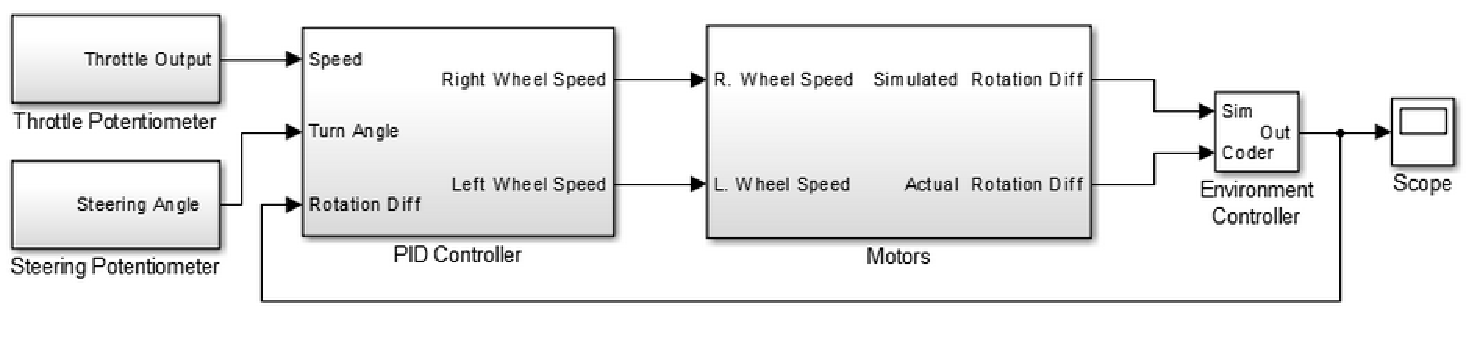
\includegraphics[scale=.4]{figures/controlblock.pdf}
			\end{figure}
		\end{block}
		\begin{block}{Control Goal}
			\begin{figure}
				\centering
				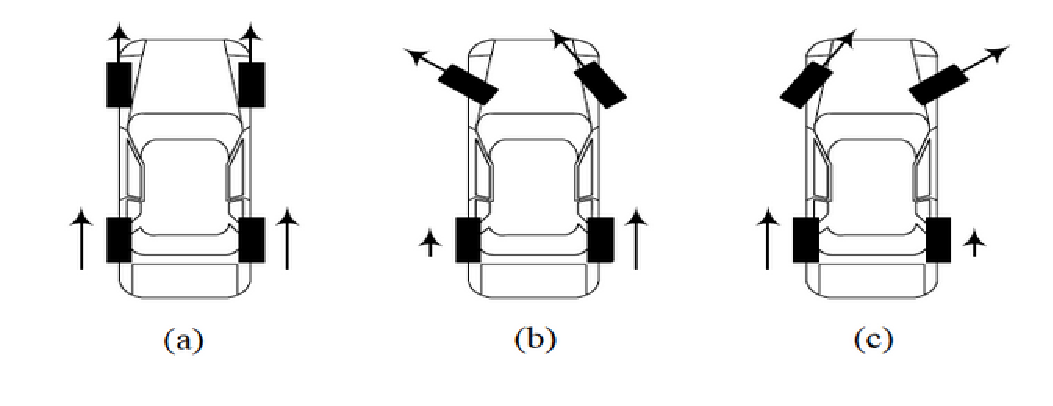
\includegraphics[scale=.4]{figures/controlgoal.pdf}
			\end{figure}
		\end{block}	
\end{frame}
%--
\begin{frame}
	\frametitle{Sensors}
		\begin{block}{Steering and Throttle}
			\begin{itemize}
				\item Potentiometers
					\begin{itemize}
						\item 5K Ohm each
						\item Analog values
						\item Used to measure rotation
					\end{itemize}
			\end{itemize}
		\end{block}
		\begin{block}{Wheel Speed}
			\begin{itemize}
				\item Encoders
					\begin{itemize}
						\item A-B Quadrature (400x / revolution)
						\item Z Pulse Absolute (1x / revolution)
						\item Max 3000 RPM (continuous) 
					\end{itemize}
			\end{itemize}
		\end{block}	
\end{frame}
%--
\begin{frame}
	\frametitle{Sensors}
	\centering
	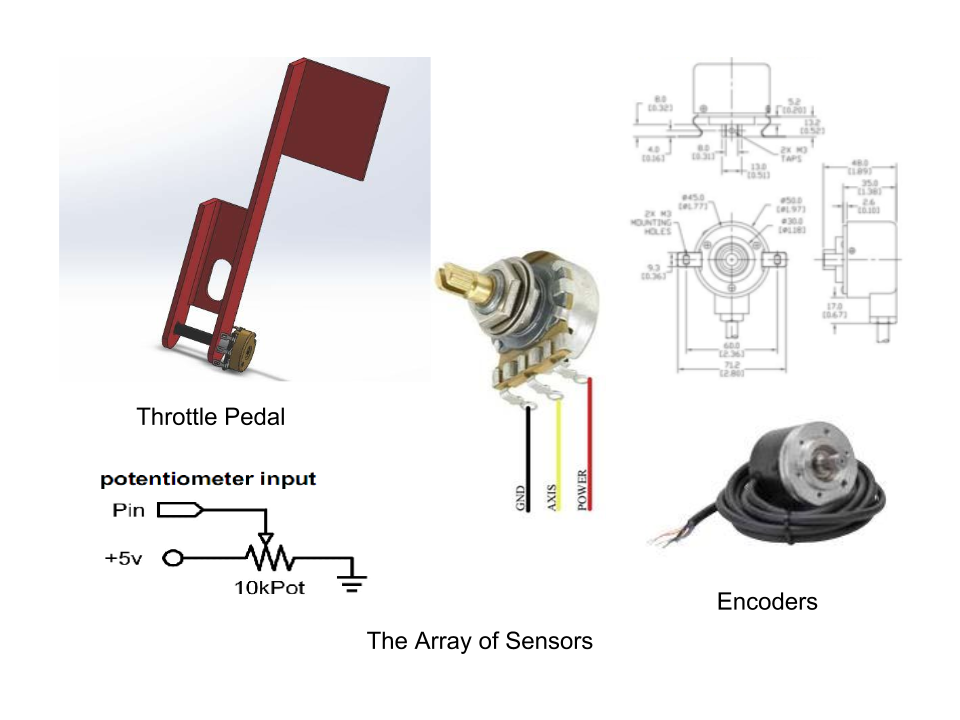
\includegraphics[scale=.3]{figures/png/SeniorDesignPresentation.png}
\end{frame}
%--
\begin{frame}
	\frametitle{Software}
		\begin{block}{Control Algorithms \& Sensor Integration}
			\begin{itemize}
				\item Throttle
				\item Steering
				\item Feedback
				\item Control Algorithms
			\end{itemize}
		\end{block}
		\begin{block}{Data Logging Programs}
			\begin{itemize}
				\item Individual Sensors
				\item Turn Radius
				\item Feedback Collection			
			\end{itemize}
		\end{block}	
\end{frame}
%--
\begin{frame}
	\frametitle{Software Control}
		\begin{block}{Github}
			\begin{itemize}
				\item Versioning
				\item Collaboration
				\item Issues
			\end{itemize}
		\end{block}
		\begin{block}{Future Students}
			\begin{itemize}
				\item Documentation
				\item Setting next year up for success
			\end{itemize}
		\end{block}	
\end{frame}
%--
\begin{frame}
	\frametitle{Throttle \& Steering Code}
		\begin{block}{Implementation}
			\begin{itemize}
				\item Reads output based on position
				\item Uses analogRead function (Arduino)
				\item Measures rotation in range of 0-1023 (integer value) based on voltage 0-3.3V 
			\end{itemize}
		\end{block}
		\begin{block}{Problems}
			\begin{itemize}
				\item Limited rotation
				\item Analog input
				\begin{itemize}
					\item Resistance vs. Capacitor Charge Time	
					\item Noise	
				\end{itemize}	
			\end{itemize}
		\end{block}	
\end{frame}
%--
\begin{frame}
	\frametitle{Encoder Code}
		\begin{block}{Implementation}
			\begin{itemize}
				\item Loop to measure pulses for given time (1/8 of second) \& Calculate time for “x” pulses
				\item Measured speed of both encoders separately
				\item Values normalized to wheel speed
			\end{itemize}
		\end{block}
		\begin{block}{Problems}
			\begin{itemize}
				\item A-B Quadrature vs. Z Absolute Pulse
				\item Speed of rotation vs. Arduino Clock Cycle
				\item Consideration of Interrupts	
			\end{itemize}
		\end{block}	
\end{frame}
%--
\begin{frame}
	\frametitle{Integration \& Control}
		\begin{block}{Process}
			\begin{enumerate}
				\item Initialize values and constants
				\item Collect sensor readings
				\item Compute control (Digital PI control scheme)
				\item Add control to running sum
				\item Apply voltage to motors based on computed control values
				\item Loop back to collect readings and repeat
			\end{enumerate}
		\end{block}
\end{frame}
%================================================================================
\section{Testing}
%--
\begin{frame}
	\frametitle{Data Collection}
	\begin{columns}[T]
		\begin{column}{0.5\textwidth}
			\begin{block}{Process}
				\begin{itemize}
					\item Employed an SD Card for data logging
					\item Code for Testing
					\begin{itemize}
						\item Throttle
						\item Steering
						\item Encoder Response
						\item Turn Radius
					\end{itemize}
					\item Could not integrate into main code due to negative effects
					\item Saved to CSV file
				\end{itemize}
			\end{block}
		\end{column}		
		\begin{column}{0.5\textwidth}
			\begin{block}{Breakout Board}
				\begin{figure}
					\centering
					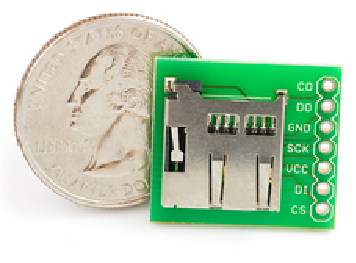
\includegraphics[scale=.9]{figures/sdcard.pdf}
				\end{figure}
			\end{block}	
		\end{column}
	\end{columns}		
\end{frame}
%--
\begin{frame}
	\frametitle{Data Logging Results}
		\begin{block}{Measured turn radius with respect to steering analog input}
			\begin{figure}
			    \centering
				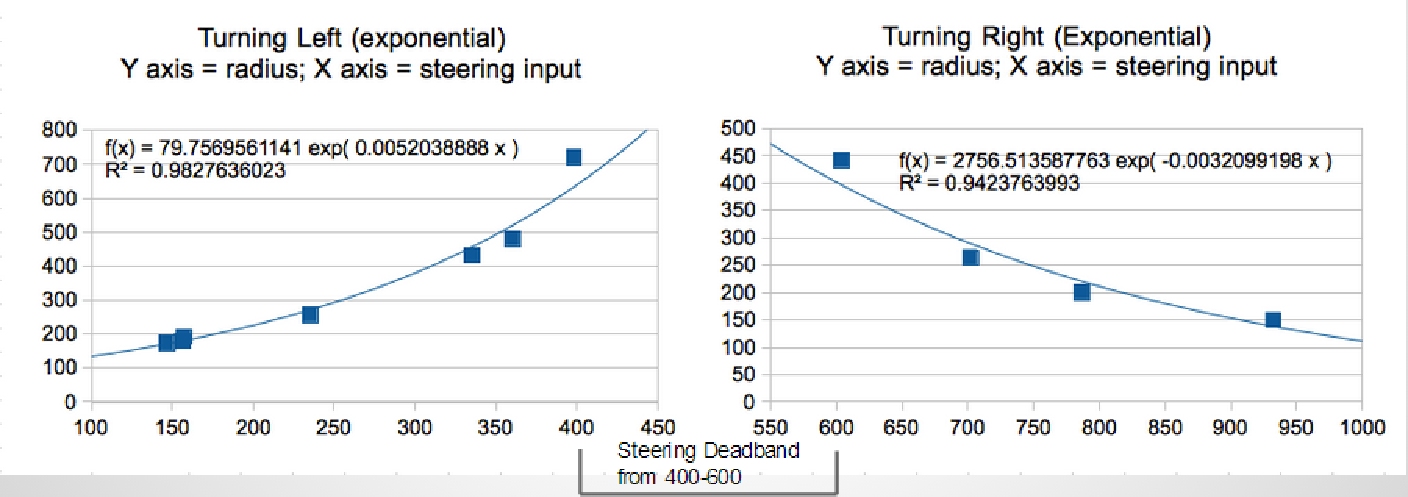
\includegraphics[scale=.45]{figures/result1.pdf}
			\end{figure}
		\end{block}
\end{frame}
%--
\begin{frame}
	\frametitle{Data Logging Results}
		\begin{block}{Accel Input to DAC Output}
			\begin{figure}
			    \centering
				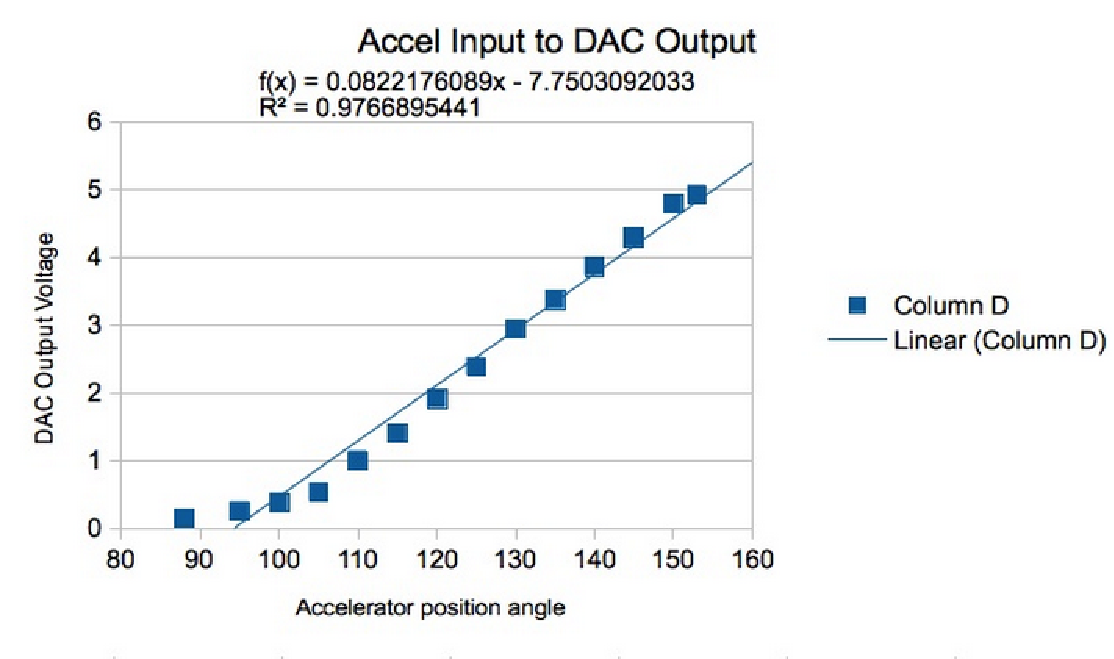
\includegraphics[scale=.5]{figures/result2.pdf}
			\end{figure}
		\end{block}
\end{frame}
%--
\begin{frame}
	\frametitle{Debugging}
		\begin{block}{Troubleshooting}
			\begin{itemize}
				\item Encoder
				\item Dissimilar motor behavior
				\item Brake behavior
				\item Multiple analog inputs
			\end{itemize}
		\end{block}
\end{frame}
%--
\begin{frame}
	\frametitle{Testing}
		\begin{block}{Process}
			\begin{itemize}
				\item The electronic differential system must show measurable improvement over a solid axle system and a forced couple system in a turning radius test. 
				\item Wheel "hopping" during solid-axle testing
			\end{itemize}
		\end{block}
\end{frame}
%--
\begin{frame}
	\frametitle{Results}
	\begin{columns}[T]
		\begin{column}{0.5\textwidth}
			\begin{block}{Outcome}
				\begin{itemize}
					\item Solid-Axle Testing
					\begin{itemize}
						\item \href{http://youtu.be/F0vOdHwFx1o}{Video of differential testing (YouTube Link)}
						\item \href{http://youtu.be/mY3hA6xaVb8}{Video of solid axle testing (YouTube Link)} 
					\end{itemize}
					\item Unmet Goals
					\begin{itemize}
						\item Traction Control
						\item Regenerative Braking
					\end{itemize}
				\end{itemize}
			\end{block}
		\end{column}		
		\begin{column}{0.5\textwidth}
			\begin{block}{Data}
				\begin{figure}
					\centering
					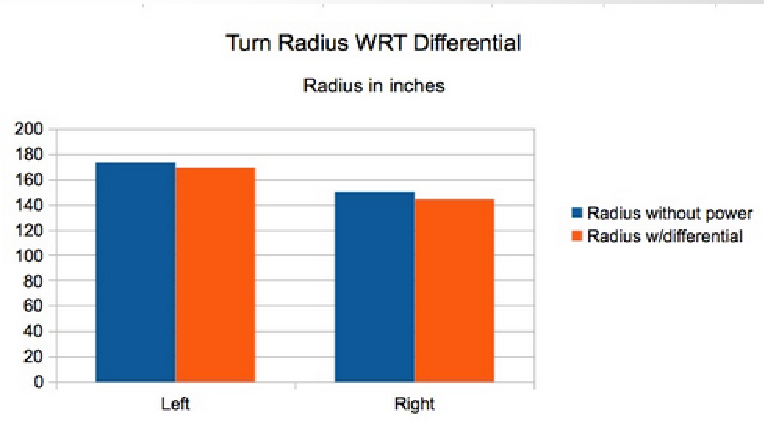
\includegraphics[scale=.4]{figures/results.pdf}
				\end{figure}
			\end{block}	
		\end{column}
	\end{columns}		
\end{frame}
%================================================================================
\section{Conclusion}
%--
\begin{frame}
	\frametitle{The Final Product}
	\begin{columns}[T]
		\begin{column}{0.5\textwidth}
			\begin{block}{Final Rendering}
				\begin{figure}
					\centering
					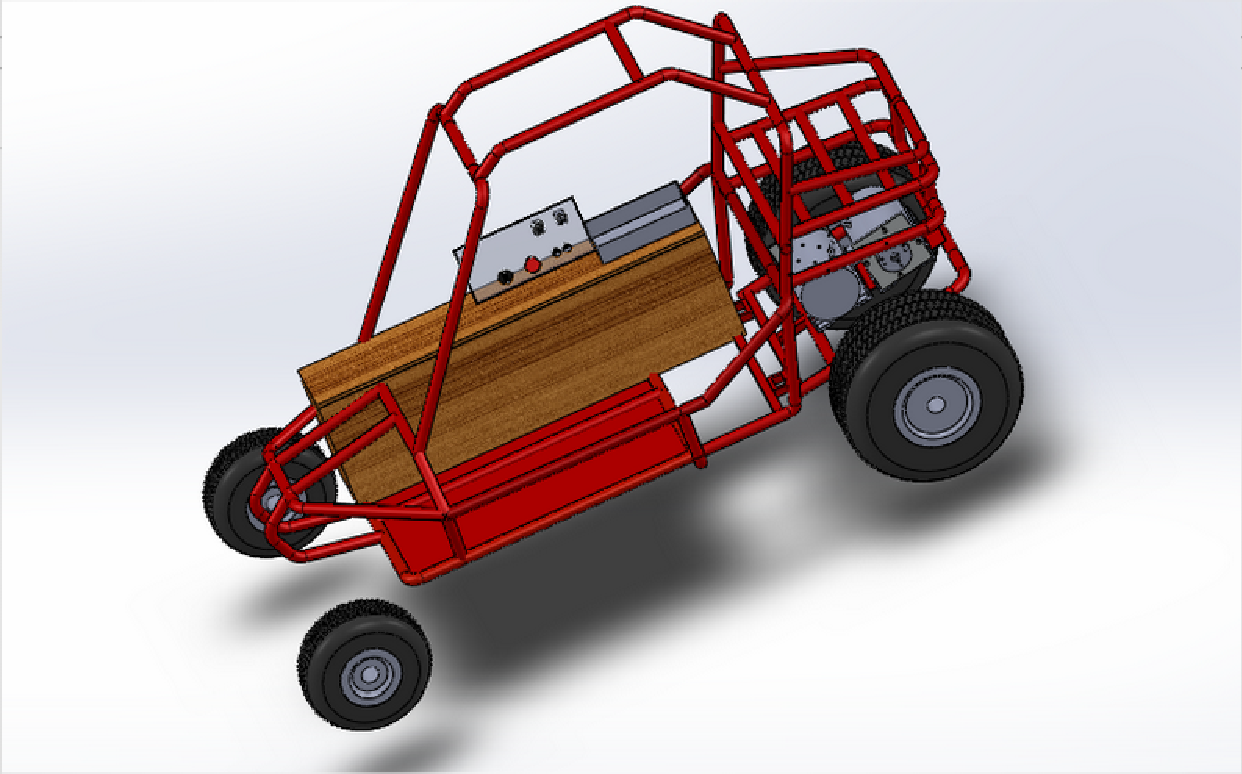
\includegraphics[scale=.25]{figures/kartfinal1.pdf}
				\end{figure}
			\end{block}
		\end{column}		
		\begin{column}{0.5\textwidth}
			\begin{block}{Finished Kart}
				\begin{figure}
					\centering
					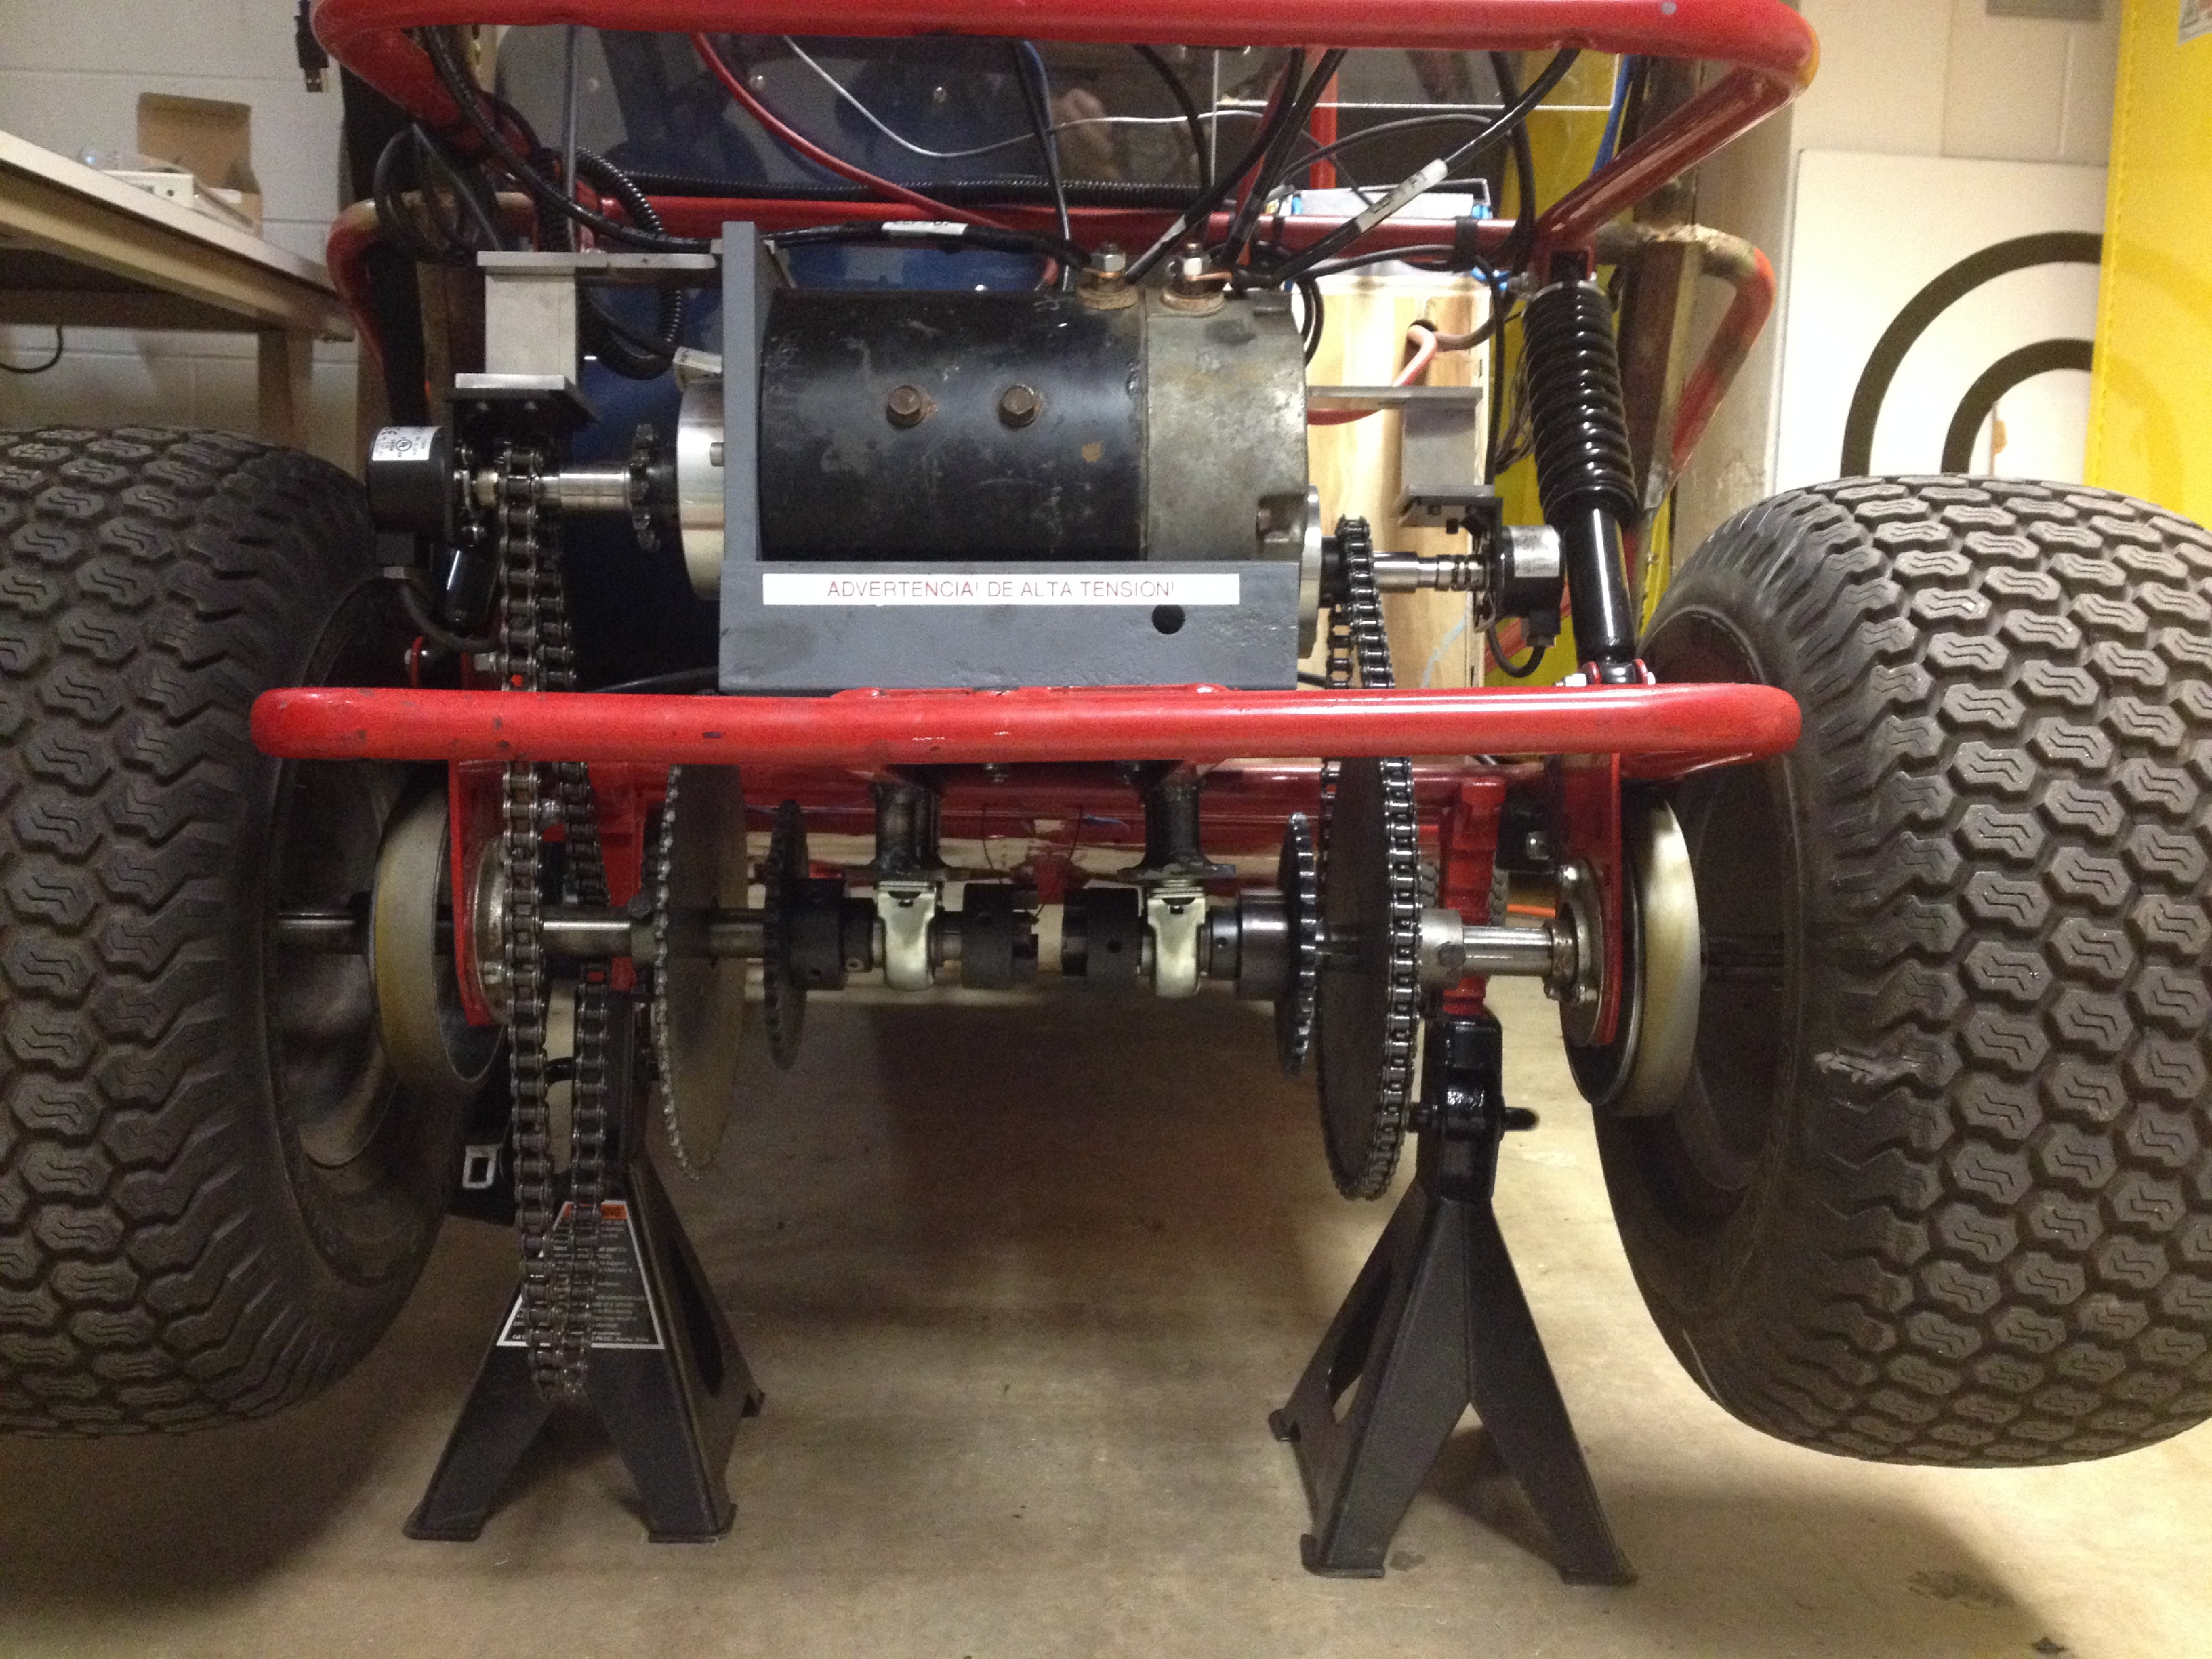
\includegraphics[scale=.03]{figures/kartfinal2.pdf}
					\\
					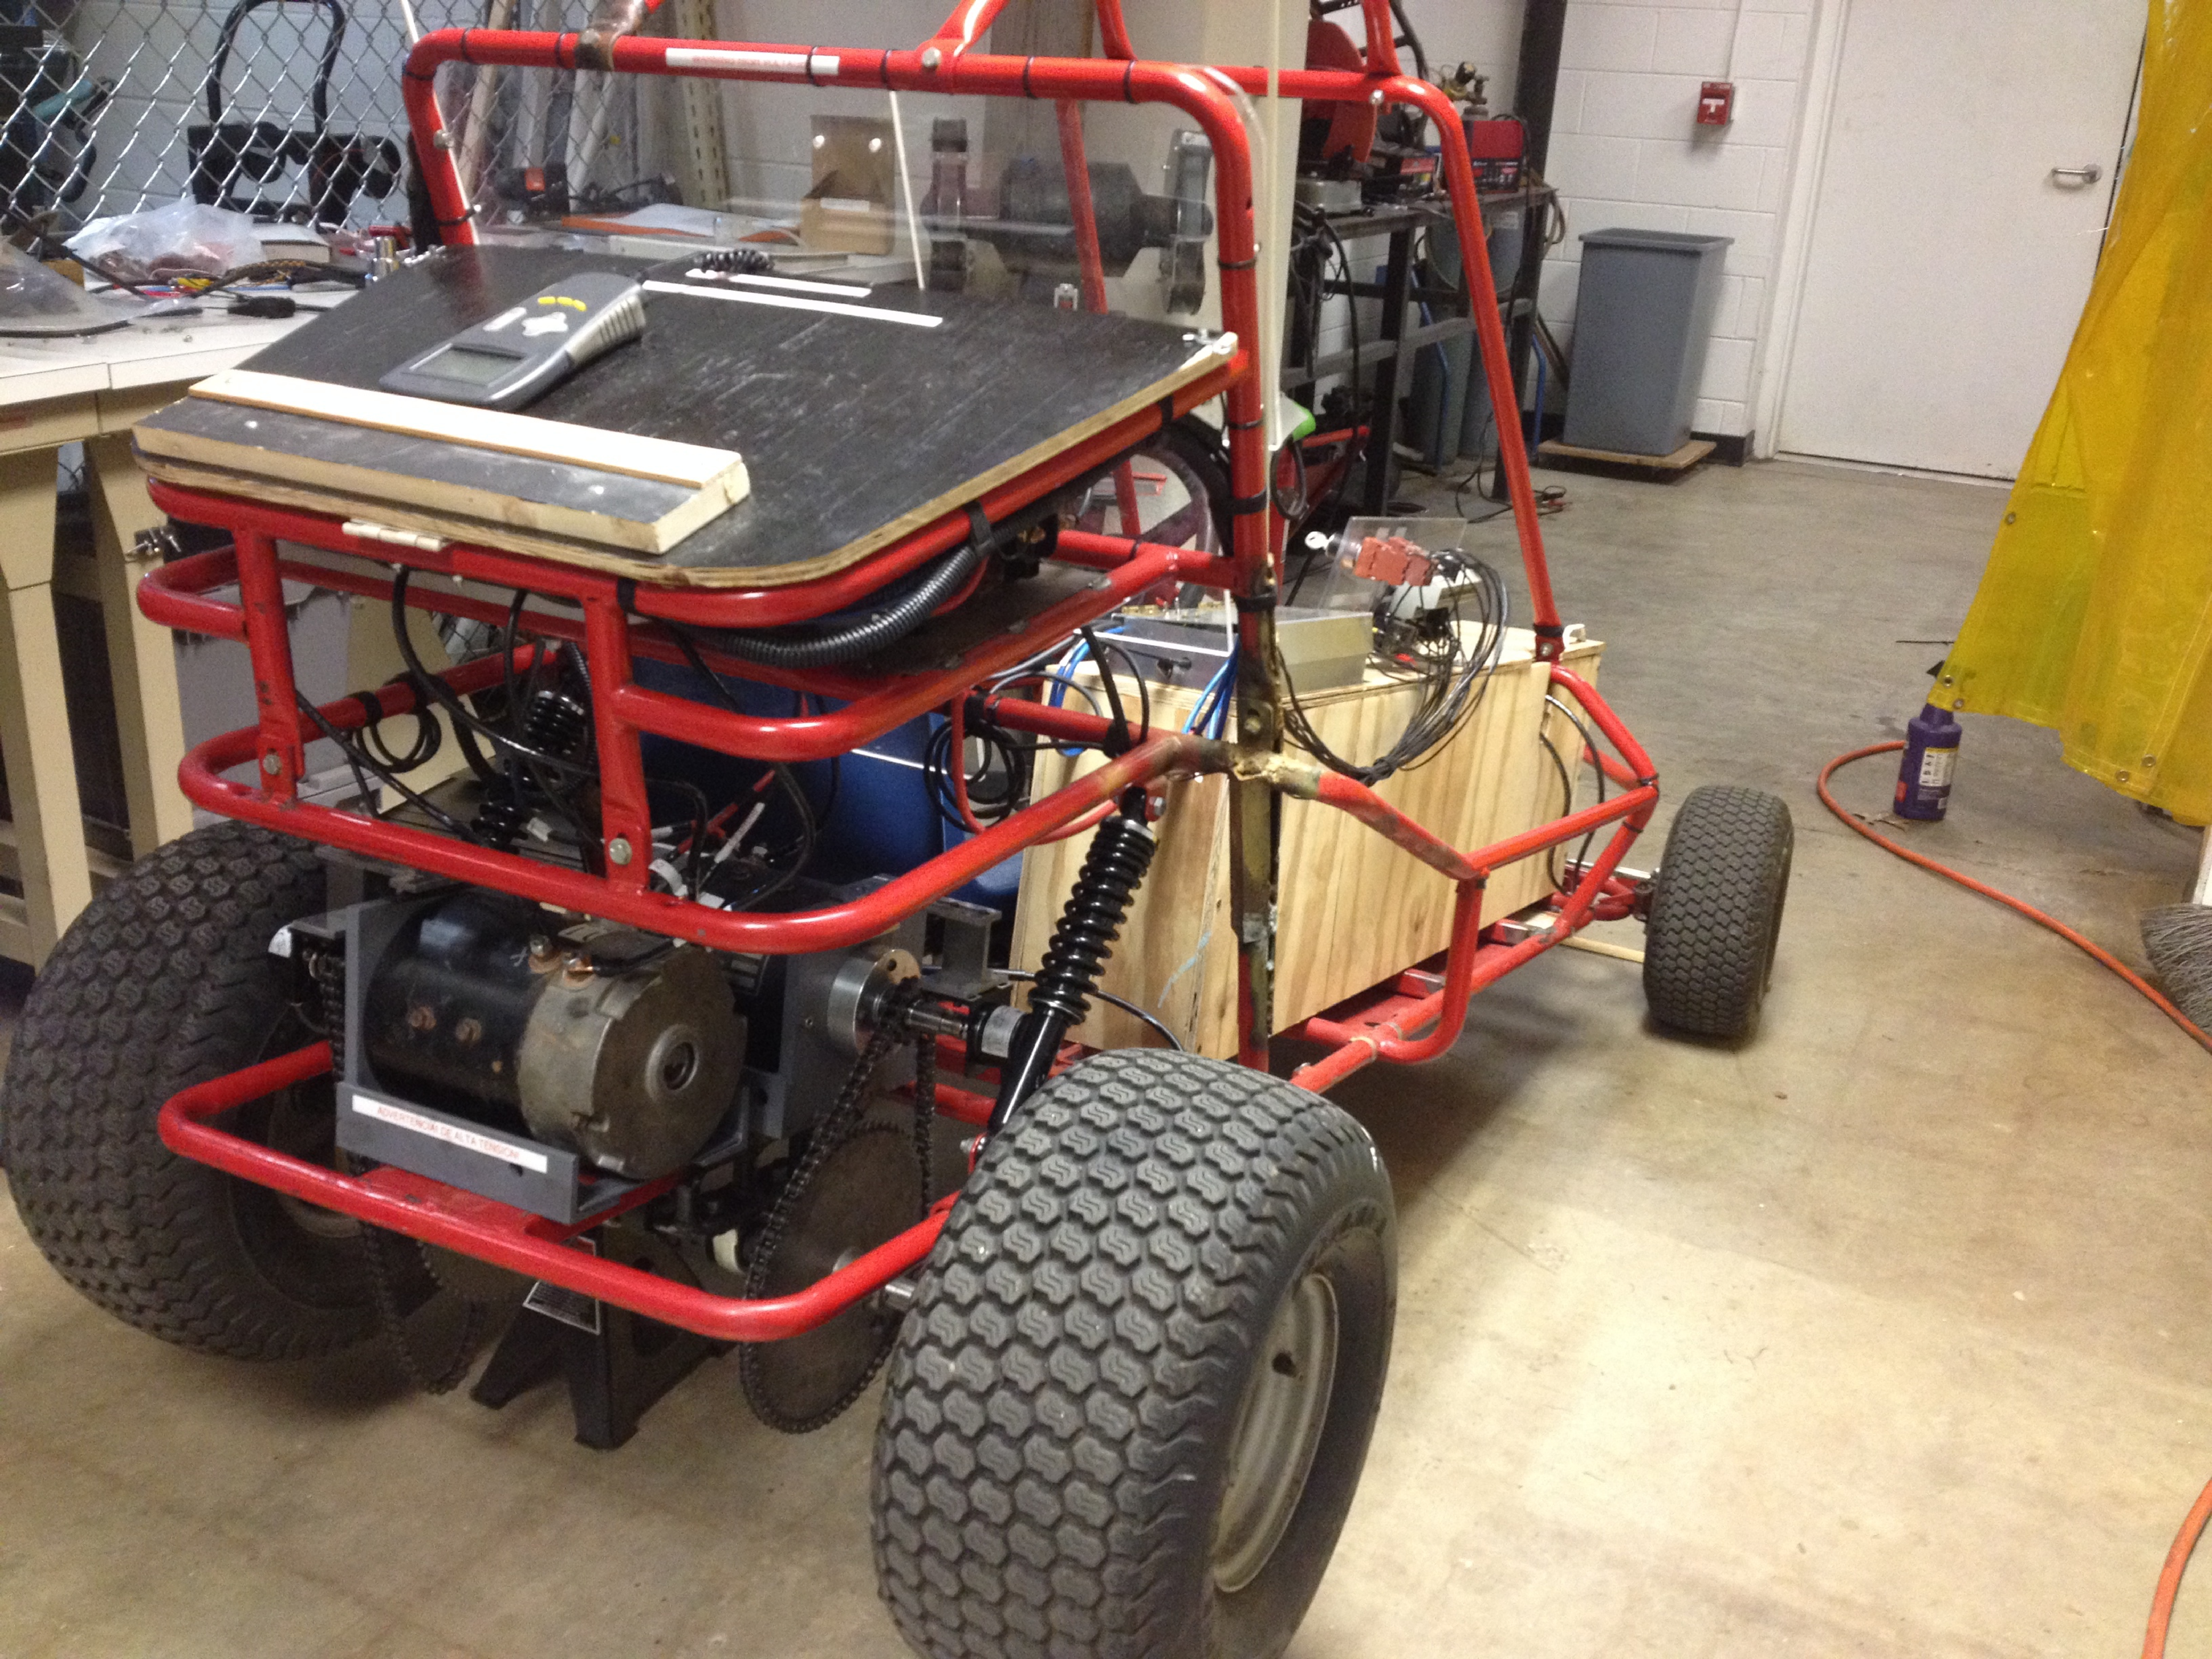
\includegraphics[scale=.03]{figures/kartfinal3.pdf}
				\end{figure}
			\end{block}	
		\end{column}
	\end{columns}		
\end{frame}
%--
\begin{frame}
	\frametitle{Conclusion}
		\begin{itemize}
			\item Successfully created a two wheel electronic differential
			\item Maintained documentation for next year
			\item The beginning of new things at UNC Asheville
		\end{itemize}
	\centering
	\includegraphics[scale=.05]{figures/group-picture.pdf} \\
Thank you for your interest and support!
\end{frame}
%================================================================================
\section{Acknowledgments}
%--
\begin{frame}
	\frametitle{Acknowledgments}
		\begin{block}{Special thanks to.....}
			\begin{figure}
			\centering
			
\includegraphics[scale=.7]{figures/thanks.pdf}
			\end{figure}
		\end{block}
\end{frame}
%================================================================================
\section{Questions}
%--
\begin{frame}
	\frametitle{Questions}
		\centering \huge Q\&A Session
\end{frame}

%================================================================================
\end{document}